\documentclass[authoryear,preprint,10pt,fleqn]{elsarticle}
\usepackage{iftex}
\ifXeTeX\else\PackageError{manuscript}{XeLaTeX or Tectonic is required}{Use the supplied compile script.}\fi
\usepackage{fontspec}
\IfFontExistsTF{Times New Roman}{\setmainfont{Times New Roman}}{\setmainfont{Liberation Serif}}
\usepackage[fontset=none]{ctex}
\IfFontExistsTF{SimSun}{\setCJKmainfont{SimSun}[AutoFakeBold=2]}{\setCJKmainfont{Noto Serif CJK SC}}
\IfFontExistsTF{Microsoft YaHei}{\setCJKsansfont{Microsoft YaHei}}{\setCJKsansfont{Noto Sans CJK SC}}
\usepackage[a4paper,margin=0.8in]{geometry}
\usepackage{graphicx}
\usepackage{amsmath,amsthm}
\usepackage{unicode-math}
\setmathfont{latinmodern-math.otf}
\usepackage{booktabs,array,tabularx,longtable,multirow}
\usepackage{enumitem}
\usepackage{microtype}
\usepackage{xurl}
\usepackage[hidelinks,unicode=true]{hyperref}
\usepackage{caption,subcaption,placeins}
\captionsetup{font=small,labelfont=normalfont,labelsep=quad,justification=justified,singlelinecheck=true}
\captionsetup[figure]{name=图}\captionsetup[table]{name=表}
\setlength{\emergencystretch}{2em}
\setlength{\mathindent}{1.5em}
\setlength{\textfloatsep}{12pt plus 2pt minus 2pt}
\setlength{\intextsep}{10pt plus 2pt minus 2pt}
\renewcommand{\topfraction}{0.9}
\renewcommand{\textfraction}{0.07}
\renewcommand{\floatpagefraction}{0.7}
\providecommand{\doi}[1]{\href{https://doi.org/#1}{\path{#1}}}
\renewcommand{\proofname}{证明}
\newtheorem{proposition}{命题}
\newtheorem{corollary}{推论}
\theoremstyle{remark}\newtheorem{remark}{注}
\newcommand{\E}{\mathbb{E}}
\newcommand{\Var}{\mathrm{Var}}
\newcommand{\Cov}{\mathrm{Cov}}
\newcommand{\Rbar}{\bar R}
\newcommand{\Rhat}{\widehat R}
\newcommand{\NB}{\mathrm{NB}}
\newcommand{\Bin}{\mathrm{Bin}}
\newcommand{\mx}{m_{\times}}
\hypersetup{pdftitle={再生数监测中推断目标与病例量的统计价值},pdfauthor={}}
% Auto-generated by experiment/code/render_revision.py; do not edit.
% Numeric-only macros. Empty definitions denote unavailable PILOT or optional inputs.
% ThinMCStatus: 1=adequate; 0=tolerance not met; -1=unavailable.
% RAaPoint <- empirical.json ["pooled", "RA", "a", "value"]
\newcommand{\RAaPoint}{0.01495}
% RAaInterval <- empirical.json ["pooled", "RA", "a", "ci95"]
\newcommand{\RAaInterval}{[0.01001, 0.02092]}
% RAbPoint <- empirical.json ["pooled", "RA", "b", "value"]
\newcommand{\RAbPoint}{0.56}
% RAbInterval <- empirical.json ["pooled", "RA", "b", "ci95"]
\newcommand{\RAbInterval}{[0.369, 0.7692]}
% RAratioPoint <- empirical.json ["pooled", "RA", "ratio", "value"]
\newcommand{\RAratioPoint}{37.44}
% RAratioInterval <- empirical.json ["pooled", "RA", "ratio", "ci95"]
\newcommand{\RAratioInterval}{[18.93, 69.92]}
% RAweekReductionPoint <- empirical.json ["centering", "RA", "week_reduction_fraction", "value"]
\newcommand{\RAweekReductionPoint}{34.7}
% RAweekReductionInterval <- empirical.json ["centering", "RA", "week_reduction_fraction", "ci95"]
\newcommand{\RAweekReductionInterval}{[5.97, 51.9]}
% RAstateCVPoint <- empirical.json ["validation", "RA", "state", "mean_score_difference"]
\newcommand{\RAstateCVPoint}{-0.002018}
% RAseasonCVPoint <- empirical.json ["validation", "RA", "season", "mean_score_difference"]
\newcommand{\RAseasonCVPoint}{0.004626}
% GaPoint <- empirical.json ["pooled", "G", "a", "value"]
\newcommand{\GaPoint}{0.08401}
% GaInterval <- empirical.json ["pooled", "G", "a", "ci95"]
\newcommand{\GaInterval}{[0.04986, 0.1234]}
% GbPoint <- empirical.json ["pooled", "G", "b", "value"]
\newcommand{\GbPoint}{1.971}
% GbInterval <- empirical.json ["pooled", "G", "b", "ci95"]
\newcommand{\GbInterval}{[0.9889, 3.042]}
% GratioPoint <- empirical.json ["pooled", "G", "ratio", "value"]
\newcommand{\GratioPoint}{23.46}
% GratioInterval <- empirical.json ["pooled", "G", "ratio", "ci95"]
\newcommand{\GratioInterval}{[8.279, 54.7]}
% GweekReductionPoint <- empirical.json ["centering", "G", "week_reduction_fraction", "value"]
\newcommand{\GweekReductionPoint}{33.3}
% GweekReductionInterval <- empirical.json ["centering", "G", "week_reduction_fraction", "ci95"]
\newcommand{\GweekReductionInterval}{[6.8, 51.6]}
% GstateCVPoint <- empirical.json ["validation", "G", "state", "mean_score_difference"]
\newcommand{\GstateCVPoint}{-0.007369}
% GseasonCVPoint <- empirical.json ["validation", "G", "season", "mean_score_difference"]
\newcommand{\GseasonCVPoint}{-0.004414}
% ThinAllPoint <- thinning.json ["estimates", "full/full/c", "value"]
\newcommand{\ThinAllPoint}{0.4051}
% ThinAllInterval <- thinning.json ["estimates", "full/full/c", "ci95"]
\newcommand{\ThinAllInterval}{[0.3656, 0.4413]}
% ThinNoqPoint <- thinning.json ["estimates", "full/noq01/c", "value"]
\newcommand{\ThinNoqPoint}{0.4848}
% ThinNoqInterval <- thinning.json ["estimates", "full/noq01/c", "ci95"]
\newcommand{\ThinNoqInterval}{[0.4387, 0.5279]}
% ThinRatioPoint <- thinning.json ["estimates", "full/full/c_over_bP", "value"]
\newcommand{\ThinRatioPoint}{0.9093}
% ThinRatioInterval <- thinning.json ["estimates", "full/full/c_over_bP", "ci95"]
\newcommand{\ThinRatioInterval}{[0.8101, 0.9995]}
% ThinHighPoint <- thinning.json ["estimates", "highCt50/full/c", "value"]
\newcommand{\ThinHighPoint}{0.4734}
% ThinHighInterval <- thinning.json ["estimates", "highCt50/full/c", "ci95"]
\newcommand{\ThinHighInterval}{[0.409, 0.5503]}
% ThinBothPoint <- thinning.json ["estimates", "both50/full/c", "value"]
\newcommand{\ThinBothPoint}{0.4926}
% ThinBothInterval <- thinning.json ["estimates", "both50/full/c", "ci95"]
\newcommand{\ThinBothInterval}{[0.42, 0.5742]}
% ThinBPPoint <- thinning.json ["estimates", "full/bP", "value"]
\newcommand{\ThinBPPoint}{0.4455}
% FEbPoint <- fixed_effects.json ["estimates", "state_b", "value"]
\newcommand{\FEbPoint}{0.3794}
% FEbInterval <- fixed_effects.json ["estimates", "state_b", "ci95"]
\newcommand{\FEbInterval}{[0.1082, 0.6403]}
% FEaPoint <- fixed_effects.json ["estimates", "a_mean", "value"]
\newcommand{\FEaPoint}{0.02192}
% FEaInterval <- fixed_effects.json ["estimates", "a_mean", "ci95"]
\newcommand{\FEaInterval}{[0.01289, 0.03502]}
% FEratioPoint <- fixed_effects.json ["estimates", "r_mean", "value"]
\newcommand{\FEratioPoint}{17.3}
% FEratioInterval <- fixed_effects.json ["estimates", "r_mean", "ci95"]
\newcommand{\FEratioInterval}{[3.315, 47.8]}
% FEpairedPoint <- fixed_effects.json ["estimates", "paired_ratio", "value"]
\newcommand{\FEpairedPoint}{2.164}
% FEpairedInterval <- fixed_effects.json ["estimates", "paired_ratio", "ci95"]
\newcommand{\FEpairedInterval}{[1.04, 7.745]}
% FEDratioPoint <- fixed_effects.json ["estimates", "state_D_ratio", "value"]
\newcommand{\FEDratioPoint}{17.71}
% FEDratioInterval <- fixed_effects.json ["estimates", "state_D_ratio", "ci95"]
\newcommand{\FEDratioInterval}{[3.267, 47.81]}
% FEpairedBlockTwoInterval <- block2.json ["estimates", "paired_ratio", "ci95"]
\newcommand{\FEpairedBlockTwoInterval}{[0.964, 8.483]}
% FEBlockTwoValid <- block2.json ["estimates", "paired_ratio", "n_finite"]
\newcommand{\FEBlockTwoValid}{1000}
% FEpairedBlockThreeInterval <- block3.json ["estimates", "paired_ratio", "ci95"]
\newcommand{\FEpairedBlockThreeInterval}{[0.9866, 8.87]}
% FEBlockThreeValid <- block3.json ["estimates", "paired_ratio", "n_finite"]
\newcommand{\FEBlockThreeValid}{999}
% Nra <- empirical.json ["pooled", "RA", "n"]
\newcommand{\Nra}{1748}
% Ngs <- empirical.json ["pooled", "G", "n"]
\newcommand{\Ngs}{1756}
% Nweeks <- empirical.json ["pooled", "RA", "weeks"]
\newcommand{\Nweeks}{42}
% Nstates <- empirical.json ["pooled", "RA", "states"]
\newcommand{\Nstates}{51}
% FEvalid <- fixed_effects.json ["estimates", "r_mean", "n_finite"]
\newcommand{\FEvalid}{999}
% FEBootstrap <- fixed_effects.json ["metadata", "bootstrap"]
\newcommand{\FEBootstrap}{1000}
% ThinBootstrap <- thinning.json ["metadata", "bootstrap"]
\newcommand{\ThinBootstrap}{1000}
% ThinPointReps <- thinning.json ["metadata", "point_reps"]
\newcommand{\ThinPointReps}{400}
% ThinInnerReps <- thinning.json ["metadata", "inner_reps"]
\newcommand{\ThinInnerReps}{50}
% ThinMCMax <- thinning.json ["monte_carlo", "metrics"]
\newcommand{\ThinMCMax}{68.44}
% ThinMCStatus <- thinning.json ["monte_carlo", "adequate"]
\newcommand{\ThinMCStatus}{1}
% CalSourcePoint <- calibration.json ["inference", "matched32_source_sd21_binomial", "RA", "v_implied"]
\newcommand{\CalSourcePoint}{0.02884}
% CalSourceInterval <- calibration.json ["inference", "matched32_source_sd21_binomial", "RA", "v_draws", "q025_50_975_finite"]
\newcommand{\CalSourceInterval}{[0.01908, 0.04027]}
% CalLegacyPoint <- calibration.json ["inference", "matched36_binomial", "RA", "v_implied"]
\newcommand{\CalLegacyPoint}{0.04}
% CalLegacyInterval <- calibration.json ["inference", "matched36_binomial", "RA", "v_draws", "q025_50_975_finite"]
\newcommand{\CalLegacyInterval}{[0.02623, 0.0562]}

\journal{Epidemics}
\begin{document}
\begin{frontmatter}
\title{再生数监测中推断目标与病例量的统计价值}
\abstracttitle{摘要}\keywordtitle{关键词}
\begin{abstract}
\noindent 本研究探讨传染病再生数估计中增加报告病例量的统计收益如何取决于推断目标。在包含环境变异、过度离散后代与二项报告的分支更新过程模型中，由 $m$ 个期望病例构建的条件无偏估计量，对当期瞬时值 $R_t$ 的均方误差为 $A/m$，但对跨期超总体过程均值 $\bar{R}$ 的单期均方误差为 $v_R+A/m$；这是因为 $R_t$ 在时期之间的真实变异构成了推断过程目标时不可消除的跨期抽样变异。未观测的动态报告波动还会引入一项不随 $m$ 下降的方差，即使对当期目标亦存在渐近方差底线；而对有限观察期的实现均值 $\bar{R}_T$，估计误差随总病例量严格衰减为 $A/(Tm)$。利用美国四个流感季早期增长期的住院数据（1748 个州周），仿射损失模型给出的条件截距为正（表观平衡比为每周 37.4 例住院，95\% CI: 19.1, 71.0），但无截距幂律模型在现有观测支持域上的拟合效果相当（$p=0.114$，交叉验证不倾向仿射形式）。受控二项稀释实验验证了计数误差项的 $1/m$ 标度律（斜率增加速率 $c=0.41$，95\% CI: 0.31, 0.53，与泊松基准 $0.45$ 相容；$q\ge0.2$ 时为 $0.48$），且排除了大幅度的截距漂移。州固定效应模型给出的州内平衡比为 17.3（95\% CI: 3.3, 51.4），与横截面比值的差异在统计上无法与抽样误差区分。基于匹配模拟的校准显示，在基准代际间隔 3.6 天代理值下潜在环境方差为 0.040（95\% CI: 0.026, 0.056），在直接测定的 2.2 至 2.9 天下为 0.013 至 0.026，且截距的 41\% 至 51\% 为同周所有州共有。这些诊断验证了计数噪声模型的标度响应，同时表明常规横截面监测数据既无法将渐近方差底线与幂律衰减经验分离，亦无法唯一识别潜在传播环境方差。
\end{abstract}

\begin{keyword}
再生数 \sep 环境随机性 \sep 监测设计 \sep 报告异质性 \sep 流感住院 \sep 推断目标
\end{keyword}

\end{frontmatter}
\section{引言}
\label{sec:intro}

再生数监测中追加病例的价值取决于所估计的量。当期传播水平、已观测区间内传播水平的平均值，以及生成连续时期的过程均值，是不同的推断目标。它们都可能服务于监测，却赋予跨期变异不同的角色。估计当期值时，传播变化属于信号；估计过程均值时，这种变化贡献抽样变异。因此，关于精度极限的陈述需要同时指明目标与观测模型，单凭病例量无法确定这一极限。

再生数概括指定条件下的传播能力，为流行态势评估提供依据\citep{fraser2007estimating, gostic2020practical}。更新方法通过代际间隔分布把发病数与既往感染压力联系起来，其不确定性取决于观测计数包含的信息\citep{cori2013new, thompson2019improved}。有关低发病率、报告噪声与及时发现传播变化的研究，已阐明逐期推断的重要限制\citep{parag2021improved, parag2022quantifying, parag2025asymmetric}。时间聚合与观测延迟又使传播过程与观测序列的表观再生数产生差异\citep{nash2023estimating, ogigittins2024simulation, eales2024differences}。这些研究促使我们区分两类不确定性：一类关于已经实现的传播轨迹，另一类关于该轨迹所抽自的时期总体。

本文在单代分枝实验中展开这一区分。原发病例独立产生负二项后代，每例继发感染独立报告，原发病例数由设计固定或外生给定。在报告概率固定且已知时，尺度化计数是当期再生数的条件无偏估计，其期望平方误差与病例量成反比。对固定的一组已观测时期取平均，若目标为这些时期的实现均值，同样可以降低计数误差。估计平稳过程均值则还需计入这些时期的抽样方差。在相同时期内增加病例不会改变这一附加项，而增加时期可以按其相依结构降低该项。

这一区分建立在经典方差结构之上。种群生态学区分个体独立结局与种群共有的环境变异\citep{engen1998demographic, lande2003stochastic}；随机流行病模型也区分种群统计贡献与环境贡献\citep{breto2009time, he2010plug}。共同条件可以包括气候、接触模式与学校校历\citep{cauchemez2008estimating, shaman2009absolute}。在抽样理论中，增加群内观测降低群内误差，增加群数则应对群间变异\citep{cochran1977sampling, hayes1999simple}。本文的贡献是为再生数监测明确对应项，并展示改变推断目标如何改变相关风险。由此得到的平衡规模是在指定模型下比较两项贡献的参照，并非普适的最低病例要求。

报告过程需要单独讨论。感染的独立漏报与同一时期所有感染共同受到的报告概率变化并不相同\citep{azmon2014estimating, stoner2019hierarchical}。即使报告概率稳定，只要其数值未知或计数归一化错误，也可能产生偏差。当报告概率独立于传播而波动时，以已知平均报告率归一化仍会给当期值估计留下额外误差；它也影响有限时期实现均值。对于过程均值，仅凭计数均值与方差一般无法分离报告波动和传播变异。这与时间序列中过程变异和观测变异难以区分的更普遍问题一致\citep{knape2008estimability, augermethe2016state}。

常规医院监测并不直接观测分枝实验中的变量。住院发生在感染之后，带有延迟，汇总了异质人群，并按日历周期记录。住院计数规模是流行过程的结果，并非外生设计变量。因此，本文考察美国国家医疗安全网络（NHSN）流感住院数据中表观周增长统计量的相对偏差平方\citep{cdc2026nhsn, frutos2025evaluation}。这些偏差描述统计量围绕经验中心的变异，并不是相对于已观测传播真值的平方误差。它们与计数倒数之间的仿射关联可以描述这种变异，却不据此识别生物学来源，也不确立观测计数范围之外的渐近极限。

实证分析区分数据能够回答的不同问题。仿射曲线与幂律曲线的比较涉及描述性形态与预测；受控二项稀释考察对既有观测轨迹追加抽样所引起的响应；州截距拟合考察州内关联，替代中心则评估共同时间模式带来的敏感性。模拟在给定代际间隔、延迟与相依结构的条件下，将这些摘要与指定的传播及观测机制联系起来。上述任何操作都不能单独识别传播环境方差。其作用、不确定性计算与执行状态在方法和结果中说明（第~\ref{sec:methods}~节与第~\ref{sec:results}~节）。

因此，本文先明确推断目标，再解释病例量的作用。第~\ref{sec:background}~节给出精确恒等式与矩不可识别结果，表~\ref{tab:targets} 汇总各目标。随后，实证分析在观测统计量尺度上评价关联及其敏感性。证明以及预测、收缩估计与设计的符号化扩展置于附录。各部分共同说明：追加病例在何种条件下改善所选估计，以及哪些剩余不确定性需要病例计数以外的信息。

\section{模型与推断目标}
\label{sec:background}

\subsection{观测尺度已知的分枝实验}
\label{sec:bg-model}

考虑由 $n\ge1$ 例原发感染构成的一代传播。给定再生数 $R_t>0$，原发病例 $i$ 独立产生负二项后代\citep{lloydsmith2005superspreading}，
\begin{equation}
  X_{i,t}\mid R_t\sim\NB\!\left(k,\frac{k}{k+R_t}\right),\qquad
  \E(X_{i,t}\mid R_t)=R_t,\quad
  \Var(X_{i,t}\mid R_t)=R_t+\frac{R_t^2}{k}.
  \label{eq:offspring}
\end{equation}
其中 $k>0$ 控制个体异质性。每例继发感染以概率 $\rho\in(0,1]$ 独立报告。求和与二项稀疏化给出
\begin{equation}
\begin{aligned}
  C_t\mid n,R_t&\sim\NB\!\left(nk,\frac{k}{k+\rho R_t}\right),\\
  \E(C_t\mid n,R_t)&=\rho nR_t,\qquad
  \Var(C_t\mid n,R_t)=\rho nR_t+\frac{\rho^2nR_t^2}{k}.
\end{aligned}
  \label{eq:observed}
\end{equation}
定义 $m=\rho n$ 和 $\Rhat_t=C_t/m$。设计规模 $m$ 是 $R_t=1$ 时的期望报告数，而非实现计数 $C_t$。

基准假设为：$\rho$ 固定已知且报告相互独立（H1）；后代在条件下独立并服从式~(\ref{eq:offspring})（H2）；$k$ 固定，且在似然计算中已知（H3）；$n$ 固定或外生给定，并与传播独立（H4）。结果以所选设计为条件，各期具有相同的 $m$。记 $\E(R_t)=\Rbar>0$、$\Var(R_t)=v_R<\infty$。对于重复时期，另假定给定完整传播轨迹后各期计数独立，且条件分布为式~(\ref{eq:observed})。这里描述的是重复分枝实验，并不主张自然演化的发病数具有外生性。

观测尺度至关重要。未知报告比例的稳定性不足以确立无偏性：若除以假定的 $\rho_0$，条件均值为 $(\rho/\rho_0)R_t$，增加病例无法消除相应的乘性偏差。由含噪观测发病数构造的比值也具有随机分母，不必具备 $C_t/(\rho n)$ 的性质。因此，基准模型是一种明确的参照实验，而不是适用于所有监测统计量的直接模型。

条件计数方差同时包含后代随机性与独立漏报。先以继发感染总数为条件，可将两者贡献分别写为 $(R_t+R_t^2/k)/n$ 和 $(1-\rho)R_t/(\rho n)$，二者之和等于上述方差。特别地，与 $R_t$ 成线性的项并不全是报告噪声：完全报告时它仍然存在。这一区分避免将纯代数分项误认为唯一的生物学归因。

\subsection{当期值、实现均值与过程均值}
\label{sec:bg-variance}

对于当期目标，$\E(\Rhat_t\mid R_t)=R_t$，条件方差为 $[R_t+\rho R_t^2/k]/m$，达到单参数计数模型中的条件 Cram\'er--Rao 下界（附录~\ref{app:proofs}）。该陈述针对在此似然下对每个 $R_t$ 都无偏的估计量，不是普适的极小极大下界，也不涵盖有偏、分层或使用先验信息的方法。

\begin{proposition}[单个时期的两个目标]
\label{prop:average}
在 H1--H4 下，令 $A=\Rbar+\rho(\Rbar^2+v_R)/k$，则
\begin{equation}
\begin{aligned}
  \E[(\Rhat_t-R_t)^2]&=\frac{A}{m},\\
  V(m):=\E[(\Rhat_t-\Rbar)^2]&=v_R+\frac{A}{m}.
\end{aligned}
  \label{eq:var-average}
\end{equation}
在仅基于当期计数且对 $R_t$ 条件无偏的估计量类中，$\Rhat_t$ 同时最小化这两种风险。
\end{proposition}

第一种风险按指定的 $R_t$ 分布对条件估计误差取平均，既不是每个固定取值下的条件风险，也不是某一时期的后验可信区间。第二种风险以不同目标评价同一个观测。单期比较只涉及边际矩，因此不要求传播时期彼此独立；跨期汇总风险时，独立性才发挥作用。

这一区别来自
\begin{equation}
  \Rhat_t-\Rbar=(\Rhat_t-R_t)+(R_t-\Rbar).
  \label{eq:error-split}
\end{equation}
条件无偏性使两项不相关。跨期传播变异属于当期信号，却为过程均值贡献抽样误差。后者是指定平稳分布下的均值，不会自动等同于非平稳流行过程的季节平均。两项贡献具有整群抽样中熟悉的单元内与单元间结构\citep{cochran1977sampling, engen1998demographic}。

当 $v_R>0$ 时，定义平衡规模 $\mx=A/v_R$。固定 $\rho$、$k$ 与传播分布，通过 $n$ 增加 $m$ 不改变 $A$；在 $m=\mx$ 处，$V(m)$ 的两项贡献相等。这一规模描述所选估计量与目标，并不意味着所有信息的丧失；改变 $\rho$ 则会同时改变 $A$ 和 $m$。覆盖与预算计算仅作为符号化扩展列于附录~\ref{app:extensions}。

\begin{corollary}[固定的一组已观测时期]
\label{cor:targets}
在 H1--H4 及给定 $R_{1:T}$ 后计数条件独立的假设下，定义 $\Rbar_T=T^{-1}\sum_{t=1}^T R_t$ 和 $\widehat{\Rbar}_T=T^{-1}\sum_{t=1}^T\Rhat_t$。对整数 $T\ge1$，若 $R_t$ 具有共同边际矩，则
\begin{equation}
\begin{aligned}
  \E[(\widehat{\Rbar}_T-\Rbar_T)^2]&=\frac{A}{Tm},\\
  \E[(\widehat{\Rbar}_T-\Rbar)^2]&=B_T+\frac{A}{Tm},
  \qquad B_T=\Var(\Rbar_T).
\end{aligned}
  \label{eq:target-means}
\end{equation}
若 $R_t$ 独立同分布，则 $B_T=v_R/T$。对满足 $\Cov(R_t,R_{t+h})=v_R\phi^{|h|}$、$|\phi|<1$ 的平稳过程，有限 $T$ 下的精确表达式为 $B_T=v_RS(\phi,T)/T^2$，其中
\begin{equation}
  S(\phi,T)=T+2\sum_{h=1}^{T-1}(T-h)\phi^h
  =\frac{T(1+\phi)}{1-\phi}-\frac{2\phi(1-\phi^T)}{(1-\phi)^2}.
  \label{eq:ar-sum}
\end{equation}
\end{corollary}

实现均值的恒等式不要求各期传播水平独立，只要求计数误差条件独立且具有所述共同矩。固定 $T$ 而增加病例，可以消除实现均值的计数误差；过程均值的风险则趋于 $B_T$。追加时期应对的是这一项，其贡献取决于相依性。预测未来值是另一个目标，见附录~\ref{app:extensions}。

平稳协方差公式使用整数时期和完整的有限求和，而非长序列近似。正的持续性通常减小相邻时期带来的收益，负自相关则可能增加收益。不能自动将序列相关过程或均值变化的流行季替换为独立抽取。对于非平稳传播，实现均值仍有明确定义，但共同过程均值的解释需要额外模型。

空间平均具有类似条件。若 $J$ 个单元的传播方差均为 $v_R$、平均两两相关系数为 $\bar c$，其等权传播均值的方差为
\begin{equation}
  \Var\!\left(J^{-1}\sum_{j=1}^J R_{j,t}\right)
  =v_R\left[\bar c+\frac{1-\bar c}{J}\right].
  \label{eq:pooling}
\end{equation}
这是协方差恒等式，并非经验回归截距的分解。方差不等、权重不等或相关结构变化时，需使用对应的协方差矩阵。

\subsection{不可观测的报告波动与识别}
\label{sec:bg-reporting}

将 H1 替换为共同的逐期报告概率 $p_t\in[0,1]$：其独立于 $R_t$ 及设计，已知均值为 $\rho>0$，且 $\Var(p_t)=\rho^2\tau^2$（H5）。给定 $p_t$ 时，各例感染仍独立报告。必有 $\tau^2\le(1-\rho)/\rho$。估计量仍除以 $m=\rho n$，并不观测 $p_t$。

\begin{proposition}[报告波动与矩不可识别性]
\label{prop:report-noise}
在 H2--H5 下，记 $Q=\Rbar^2+v_R$，则
\begin{equation}
\begin{aligned}
  \E(\Rhat_t)&=\Rbar,\qquad
  V_H(m):=\Var(\Rhat_t)=v_R+v_H+\frac{A_H}{m},\\
  v_H&=\tau^2Q,\qquad
  A_H=\Rbar+\frac{\rho(1+\tau^2)Q}{k}.
\end{aligned}
  \label{eq:vH-AH}
\end{equation}
当 $m$、$\rho$ 和 $k$ 已知时，计数的前两个矩仅通过 $U=(1+\tau^2)(\Rbar^2+v_R)$ 依赖 $v_R$ 与 $\tau^2$，因此一般不能分别识别传播方差与报告波动。
\end{proposition}

同时给定 $R_t$ 与 $p_t$ 时，估计量的均值为 $(p_t/\rho)R_t$。只有对均值正确且独立的报告过程取平均后，才恢复对 $R_t$ 的无偏性。这说明为何同一时期内增加感染数无法平均掉共同报告冲击。如果能测量当期报告概率且它为正，正确调整的估计量将对应另一个问题；测量该概率的不确定性本身也需要传播。

这是指定模型族中的矩不可识别结果，并不意味着外部报告测量、附加假设下的时间信息，或限制更强的完整分布永远无法识别机制。边界情形也可能带来进一步约束。报告与传播独立是一项实质性条件；若疾病负担改变报告实践，上述分解未必成立。

\begin{corollary}[报告波动下的当期值与实现均值风险]
\label{cor:report-current}
在 H2--H5 下，
\begin{equation}
  \E[(\Rhat_t-R_t)^2]=v_H+\frac{A_H}{m}.
  \label{eq:vH-current}
\end{equation}
若另外假定各期 $p_t$ 独立同分布、独立于完整传播轨迹，且给定两条轨迹后各期计数独立，则
\begin{equation}
  \E[(\widehat{\Rbar}_T-\Rbar_T)^2]=\frac{v_H+A_H/m}{T},\qquad
  \E[(\widehat{\Rbar}_T-\Rbar)^2]=B_T+\frac{v_H+A_H/m}{T}.
  \label{eq:report-means}
\end{equation}
\end{corollary}

因此，实现目标中没有传播变异项，不代表没有报告误差。固定 $T$ 时，随着 $m$ 增加，不可观测的报告波动仍然存在。报告的序列相依性会增加协方差项，稳定但未知的平均报告比例也会引入偏差。表~\ref{tab:targets} 汇总了各恒等式及其条件。

\begin{table}[t]
\centering
\small
\setlength{\tabcolsep}{4pt}
\caption{推断目标及精确均方误差。固定报告列假设 H1--H4；波动报告列假设 H2--H5，且对跨期均值另要求各期报告概率独立、独立于完整传播轨迹。各期计数误差条件独立。$B_T=\Var(\Rbar_T)$；传播独立同分布时等于 $v_R/T$，具有所述平稳自协方差时等于 $v_RS(\phi,T)/T^2$。}
\label{tab:targets}
\begin{tabularx}{\linewidth}{>{\raggedright\arraybackslash}X>{\centering\arraybackslash}p{0.16\linewidth}>{\centering\arraybackslash}p{0.24\linewidth}>{\centering\arraybackslash}p{0.27\linewidth}}
\toprule
目标 & 估计量 & 固定且已知的报告 & 不可观测的波动报告 \\
\midrule
当期值 $R_t$ & $\Rhat_t$ & $A/m$ & $v_H+A_H/m$ \\
实现均值 $\Rbar_T$ & $\widehat{\Rbar}_T$ & $A/(Tm)$ & $(v_H+A_H/m)/T$ \\
过程均值 $\Rbar$ & $\widehat{\Rbar}_T$ & $B_T+A/(Tm)$ & $B_T+(v_H+A_H/m)/T$ \\
\bottomrule
\end{tabularx}
\end{table}

\subsection{内生计数规模与表观统计量}
\label{sec:bg-scope}

若 $m=\rho n$ 随机且与传播关联，即使保留给定 $(R_t,m)$ 的条件计数分布与无偏性，也只能得到
\begin{equation}
\begin{aligned}
 \E[(\Rhat_t-\Rbar)^2\mid m]
 &=\frac{\E(R_t\mid m)+\rho\E(R_t^2\mid m)/k}{m}\\
 &\quad+\Var(R_t\mid m)+[\E(R_t\mid m)-\Rbar]^2.
\end{aligned}
\label{eq:endogenous-risk}
\end{equation}
这些条件矩可能随规模改变，因此推不出常数截距加常数系数乘计数倒数的形式。以观测到的结果计数为条件，限制更强：这种条件化未必保留原先假定的条件观测分布。仅采用更新方程表述并不能解决上述任何问题。

因此，实证响应定义为表观统计量相对于指定中心的相对偏差平方（第~\ref{sec:meth-stats}~节），而非相对于已知 $R_t$ 的误差。其仿射截距和斜率不必等于 $v_R/\Rbar^2$ 与 $A/\Rbar^2$。延迟、聚合、分母噪声与变化的条件均值都会影响这一映射。校准规定的是依赖模型的联系（第~\ref{sec:meth-inversion}~节），不会把经验截距变成生物学来源的精确加性分解。

\section{材料与方法}
\label{sec:methods}

\subsection{数据、窗口与经验目标}
\label{sec:meth-data}

使用 2026 年 10 月 20 日检索的美国国家医疗保健安全网络（NHSN）每周呼吸道住院数据快照，流感分析限于 50 州和哥伦比亚特区\citep{cdc2026nhsn,frutos2025evaluation}，排除全国、区域汇总及领地。医院参与率在观测期内变化，其中 2024 年 5--10 月为自愿报告期，之后恢复报告要求\citep{cms2024reporting}。本文描述该监测系统，不估计制度变动的因果效应。

主窗口保留此前披露的四个流感季早期增长阶段：2022 年 10 月 1 日至 11 月 26 日、2023 年 10 月 7 日至 12 月 23 日、2024 年 11 月 9 日至 12 月 28 日、2025 年 10 月 4 日至 12 月 27 日。每个窗口是该季允许起点后、第一个全国转折点之前，全国周增长不低于 1.05 的连续片段；2024 年起点在恢复强制报告后。窗口规则与主统计量已在先前分析轮次中选择，本轮修订不是预注册研究。我们固定这些窗口，而未重新选择有利于正截距的片段。推断以已选窗口为条件。

从原始快照重建观测，缺失或抑制值保持缺失，不按零住院处理；真实零计数保留。一行观测要求分母周之前两周至下一周的四个计数均存在，且日期严格按七天连续。加权病例规模需满足 $D_t\ge5$，主单周统计量还要求 $C_t\ge5$。得到 $R_A$ 的 \Nra{} 个州周与 $G$ 的 \Ngs{} 个州周，覆盖 \Nstates{} 个辖区、\Nweeks{} 个日历周。样本差异由分母条件决定。稀释之前固定州周键及原始计数。

\subsection{表观统计量与相对平方偏差}
\label{sec:meth-stats}

令 $C_t$ 表示第 $t$ 周住院数。加权增长统计量为
\begin{equation}
G_t=\frac{C_{t+1}}{D_t},\qquad D_t=0.65C_t+0.25C_{t-1}+0.10C_{t-2},
\label{eq:dt}
\end{equation}
增长率到再生数的变换为
\begin{equation}
R_{A,t}=\left[1+\frac{\theta}{7}\log\frac{C_{t+1}+0.5}{C_t+0.5}\right]_{+}^{\alpha},\qquad
\alpha=(g_\mu/g_\sigma)^2,\quad\theta=g_\sigma^2/g_\mu.
\label{eq:ra}
\end{equation}
正部约定使底数非正时仍有数值定义，并不意味着指数增长近似在此成立。伽马间隔映射来自增长率与再生数的更新关系\citep{wallinga2007how}。两个统计量都不是真实再生数的观测值，也不是感染更新模型给出的后验估计\citep{cori2013new,eales2024differences}。

为保持历史可比性，主变换采用 $g_\mu=3.6$ 天、$g_\sigma=1.6$ 天，即 \citet{cowling2009estimation} 的家庭序列间隔估计。这是代际间隔代理值。敏感性分别采用均值 3.2 天并固定原变异系数，以及均值 3.2 天、标准差 2.1 天；后者是 \citet{chan2025estimating} 表 2 的内禀代际间隔估计。固定变异系数是本文假设。家庭内实现代际间隔和亚型序列间隔是不同测量对象\citep{chan2025estimating,vink2014serial}。

每个设定计算
\begin{equation}
L_{st}=\left(\frac{X_{st}-\bar X}{\bar X}\right)^2,
\qquad E(L_{st}\mid D_{st})=a+b/D_{st},
\label{eq:affine}
\end{equation}
其中 $X$ 为表观统计量，$\bar X$ 为合并均值。对于 $R_A$，回归中的 $D_t$ 替换为 $C_t$。响应量衡量相对于拟合参照的离散程度，不是围绕已知真实 $R_t$ 的估计误差平方。$b/a$ 有定义时，描述该统计量病例尺度上的仿射工作模型，并不直接等于潜在平衡规模 $\mx$。

\subsection{拟合、不确定性与模型比较}
\label{sec:meth-inference}

采用迭代可行广义最小二乘（FGLS）拟合仿射均值，精度权重与拟合均值平方的倒数成比例。截距与斜率可以有正负号，但观测行上的拟合均值必须为正。阻尼更新使伽马准偏差目标 $\sum_iw_i[L_i/\mu_i+\log\mu_i]$ 下降；必要时的数值备用求解仍使用同一目标及正拟合均值约束。记录收敛性、秩与失败情况，达到迭代上限不作为有效估计。该目标是估计准则，不表示经验损失服从伽马分布。

主合并区间使用 2000 次州 $\times$ 日历周鸽巢自助抽样\citep{owen2007pigeonhole}。行权重为独立抽取的州与周多重性乘积，每次重新估计中心和回归；次要分析采用 1000 次抽样。另结合州多重性，在各季内按两周、三周连续块抽样，以检查全国共同冲击持续性的影响。四个季节不足以支持对任意未来流行机制的无约束外推。未定义比值、分母符号和拟合失败均保留诊断；若区间仅由有限有效重复计算，明确标注。

通过逐州留一与逐季留一比较仿射均值和 $\lambda D^{-\gamma}$。响应中心仅由训练观测计算，测试损失围绕训练中心构造；两个模型也仅在训练折内拟合。测试评分为 $L/\mu+\log\mu$ 的均值，并保留平方预测误差作为次要指标。报告幂律评分减去仿射评分，正值有利于仿射模型。训练集重叠的折不是独立重复，也不以仅四个流感季构造过度精确的显著性检验。此前残差自助平台检验的 $p$ 值不作为已修复检验继续沿用。

\subsection{受控二项稀释}
\label{sec:meth-thinning}

在 $q\in\{0.8,0.6,0.5,0.4,0.3,0.2,0.1\}$ 下，每个唯一州周计数每次从 $\operatorname{Bin}(C,q)$ 抽取一次，所有相邻比值复用该值；不重新应用筛选条件或窗口。重新计算统计量、中心和仿射拟合，回归尺度仍是原始 $C_t$。点响应平均 \ThinPointReps{} 次分别拟合的实现；\ThinBootstrap{} 次外层自助样本中，每水平平均 \ThinInnerReps{} 次内层拟合。若估计的蒙特卡洛标准误超过预先规定的样本不确定性比例，统一增加内层次数；报告实际预算与剩余模拟误差。

近似关系为
\begin{equation}
b(q)-b(1)\simeq c_{\rm thin}(1/q-1).
\label{eq:thinning}
\end{equation}
估计过原点的响应斜率，保留各水平，并分别剔除 $q=0.1$ 和逐一剔除其他水平。预定子样本要求原始 $C_t\ge50$，或同时要求 $C_t,C_{t+1}\ge50$；这限制的是稀释计数期望，而非每次实现。参照系数为 $\kappa(g)^2[1+(C_t+0.5)/(C_{t+1}+0.5)]$ 的加权均值，其中 $\kappa(g)=(g_\mu/7)/[1+\theta\log(g)/7]$、$g=(C_{t+1}+0.5)/(C_t+0.5)$。该表达式近似变换的相对响应，并稳定倒数计数，不是重新中心化后非线性统计量的精确方差。每次重抽样重新计算参照值，以形成配对 $c_{\rm thin}/b_P$ 区间；用同时区间带描述截距差向量。已知泊松计数例经过同一流程，仅用于机制检查，不作为区间覆盖率验证。

\subsection{州异质性与参照敏感性}
\label{sec:meth-fe}

保持同一合并损失定义，拟合 $E(L_{st}\mid C_{st})=a_s+b_{\rm w}/C_{st}$。州摘要以抽中的州出现次数为目标：重复抽中的州重复计入，未抽中的州不以零系数参加平均；行和病例加权摘要使用重抽样总量。合并与州内模型在同一自助样本中配对比较。分母敏感性单独把 $C_t$ 换成实际的加权 $D_t$。仅周和州加周模型作为数值诊断，失败拟合明确记为不可用。

另一组分析改变损失参照，分别使用季均值、各季内所有州共享的线性时间趋势、全国周均值，以及排除自身州的全国周均值。统一保持全局均值平方作为归一化分母，以区分中心改变与尺度改变；中心和趋势在自助样本中重估。这些操作改变经验目标，也可能移除真实传播信号，因此截距差是定义敏感性，不是正交生物学方差分解。另报告有符号相对偏差 $d=X/\bar X-1$ 的 $\operatorname{Var}_w(\bar d_w)/\operatorname{Var}_{st}(d_{st})$，明确称为描述性方差比，而不称平方损失的 ICC。

\subsection{条件校准与设计示例}
\label{sec:meth-inversion}

日度更新模拟器保持四个固定窗口长度及各州初始计数。传播采用独立负二项后代，周度再生数冲击区分全国和州分量，并声明其边际方差及持续性；住院延迟和报告概率除有外部依据者外均列为假设。二项住院事件按延迟分配；另一观察模型直接从潜在延迟住院强度 $\lambda$ 生成计数，条件均值为 $\lambda$、条件方差为 $\varphi\lambda$，不对已经带噪声的住院数再次抽样。$\varphi=1$ 为泊松极限，单独的观察矩测试检查该定义。

模拟面板使用与实证相同的统计量、筛选和拟合函数。方差参数描述该模拟器中的周度再生数冲击，不换算成每代方差或操作性周病例门槛。联合经验截距抽样和联合模拟面板重抽样传播样本与校准蒙特卡洛不确定性。不同代际间隔及观察模型情景表示结构敏感性，不是机制的后验分布，也不是覆盖全部机制的联合置信区间。补充方法列出全部设定、边界和模拟诊断；另报告分季、医院参与率敏感性以及明确假设下的曲线辨别设计实验，不将其用于报告制度因果效应或普适监测样本量推断。

\section{结果}
\label{sec:results}

\subsection{已知真实值下的目标特异风险}
\label{sec:res-theory}

已知真实值的模拟呈现了模型预言的目标差异（图~\ref{fig:concept}）。报告概率固定且正确已知时，当期再生数的误差随病例量倒数下降；固定一组已实现时期的均值误差也下降，因为这些时期的真实波动属于目标本身。对于平稳过程均值，在抽取时期数固定时，误差保留实现均值的方差。模拟仅检查模型自身假设下的公式，并不证明住院统计量截距有相同来源。

采用平均报告率归一化、而当期完整度独立波动时，当期误差趋向报告项而非零。有限时期均值也继承除以独立时期数的报告分量。因此，没有环境底线不等于没有观察过程底线。模拟记录每项比较的蒙特卡洛标准误，按模拟不确定性评价数值差异，而不以任意百分比作为一致标准。附录~\ref{app:extensions} 的方差平衡和预算结果属于该指定模型，不是由住院数据识别的操作门槛。

\begin{figure}[tbp]
\centering
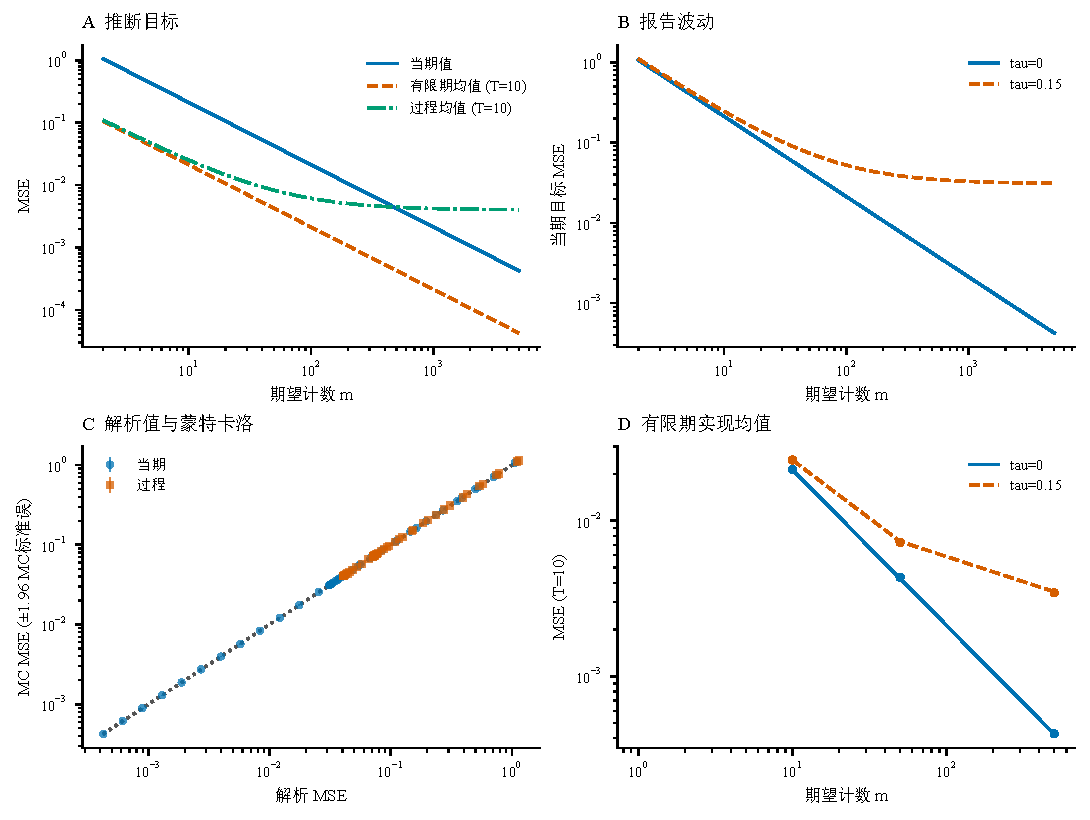
\includegraphics[width=\linewidth]{figures/fig_01_targets.pdf}
\caption{推断目标与报告假设。曲线为模型风险，图中点为已知真实值的蒙特卡洛检查。当期值和有限时期实现均值不同于平稳过程均值；不可测的时期报告波动也可给当期值留下非零风险。计数由声明的固定暴露模型生成，不代表在医院数据中识别出传播方差底线。}
\label{fig:concept}
\end{figure}

\subsection{观测损失曲线与留出比较}
\label{sec:res-empirical}

重建后的主 $R_A$ 样本包含 \Nra{} 个州周。仿射工作模型得到 $a=\RAaPoint{}$（95\% 区间 \RAaInterval{}）、$b=\RAbPoint{}$（\RAbInterval{}）及表观比值 $b/a=\RAratioPoint{}$（\RAratioInterval{}）。$G$ 的对应比值为 \GratioPoint{}（\GratioInterval{}；表~\ref{tab:pooled}）。这些估计描述指定仿射形式下表观统计量的相对离散程度；正条件截距不确定观测病例范围之外的曲线形式。

两个工作模型都描述了支持范围内损失的大体变化，但留出预测排名并不一致（图~\ref{fig:model-comparison}；表~\ref{tab:cv}）。$R_A$ 的幂律减仿射平均评分，在逐州留出时为 \RAstateCVPoint{}，逐季留出时为 \RAseasonCVPoint{}：前者为负，有利于幂律；后者为正，有利于仿射。$G$ 的两项摘要均有利于幂律，分别为 \GstateCVPoint{} 和 \GseasonCVPoint{}。比较全程使用训练折中心。各折结果单独保留，因为较小的汇总差异掩盖了留出情景之间的变化，仅四个季节也只能有限评价新流行机制中的泛化。

正拟合截距与这种混合预测排序都没有独立确立不变的传播方差平台。因此，$b/a$ 仅作为仿射描述量。表~\ref{tab:pooled} 的 3.2 天变换敏感性区分了表观统计量定义改变与模拟器真实间隔改变，不能据此判定住院数据由哪个间隔生成。补充设计实验评价声明的合成曲线之可区分性；部分设定下较高功效不能替代实证检验，零假设留出拒绝率与功效一并报告。

\begin{figure}[tbp]
\centering
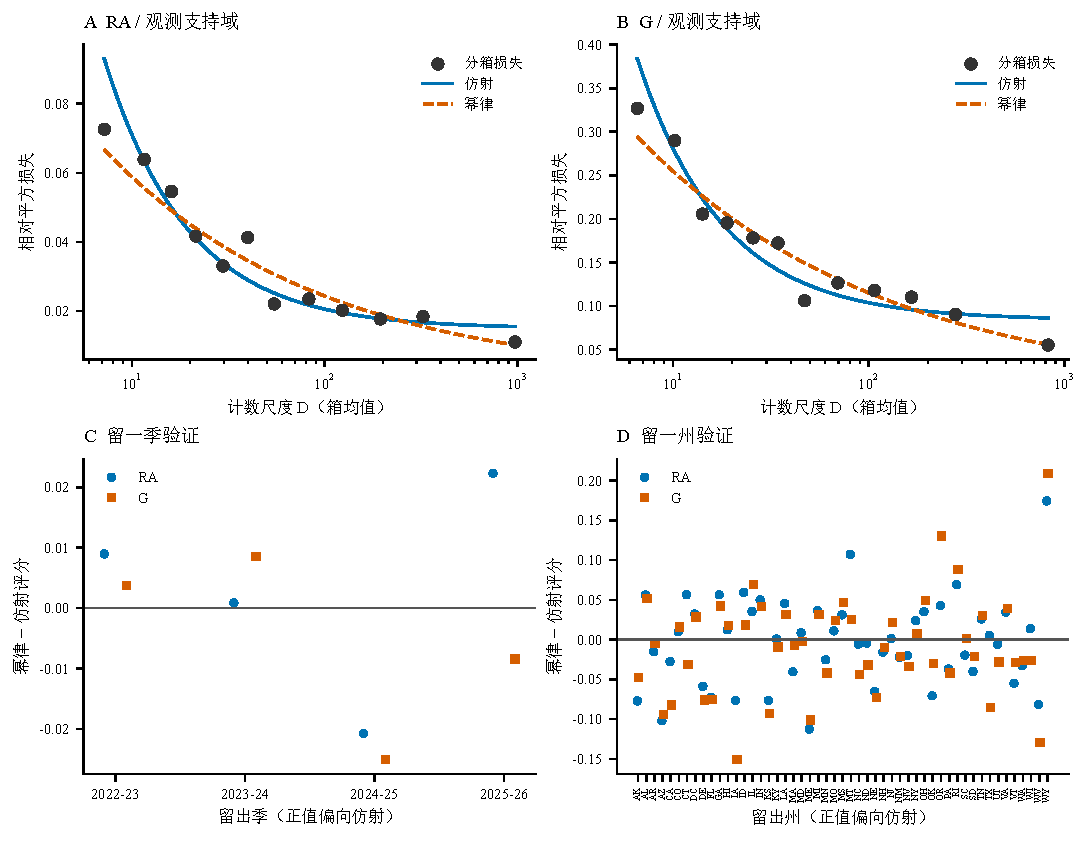
\includegraphics[width=\linewidth]{figures/fig_02_models.pdf}
\caption{经验支持范围与留出曲线比较。分箱均值描述观测病例量范围内的相对损失，不作为独立观测或未聚类显著性检验。仿射与幂律均为拟合工作模型。测试评分使用训练折内估计的中心和模型参数，幂律减仿射评分为正时有利于仿射，为负时有利于幂律。各折不是独立重复。}
\label{fig:model-comparison}
\end{figure}

\subsection{对受控随机移除病例的响应}
\label{sec:res-thinning}

对 $R_A$ 样本（n=\Nra{} 个州周），全保留率水平的稀释速率为 \ThinAllPoint{}（95\% 区间 \ThinAllInterval{}），近似弹性参照为 \ThinBPPoint{}，与参照的配对比值为 \ThinRatioPoint{}（\ThinRatioInterval{}）。剔除最极端保留率后得到 \ThinNoqPoint{}（\ThinNoqInterval{}；图~\ref{fig:thinning}、表~\ref{tab:thinning}）。二者值得并列考察，因为 $q=0.1$ 对过原点回归预测变量平方和的贡献约为 76\%。这来自所选逆保留率设计，本身不证明该点存在偏差。

原始 $C_t\ge50$ 子样本的速率为 \ThinHighPoint{}（\ThinHighInterval{}），同时要求当前和下一周计数均不低于 50 时为 \ThinBothPoint{}（\ThinBothInterval{}）。后一限制处理了前一限制的不足：较大的当前计数不保证稀释后的分子也足够大。所有子样本均由原始计数确定，不在稀释后重新筛选；每个子样本使用重新计算的参照系数，不借用全样本值。

图~\ref{fig:thinning} 同时报告截距差及联合不确定性，包括低保留率下的偏离。区间包含零不表示截距严格不变。即使施加的计数移除机制已知，非线性变换、连续性修正、重新中心化与回归仍可影响拟合响应。补充输出中的已知泊松计数例检查完整流程，不声称代表现实中的全部报告机制。

计算实际使用 \ThinBootstrap{} 次外层样本、\ThinPointReps{} 次点实现，每个外层水平使用 \ThinInnerReps{} 次内层实现。表~\ref{tab:thinning} 报告预定蒙特卡洛检查及拟合失败，由于点估计平均的实现次数多于每个自助抽样，区间同时包含抽样变异与有限内层模拟波动；表~
ef{tab:thinning} 报告两部分误差、预定蒙特卡洛检查与拟合失败。实验刻画这些已记录病例对进一步随机移除的响应，不分离原截距中的传播、住院实践、延迟观察和报告变异；$b(1)$ 与 $c_{\rm thin}$ 的差额也不唯一量化后代过度离散。

\begin{figure}[tbp]
\centering
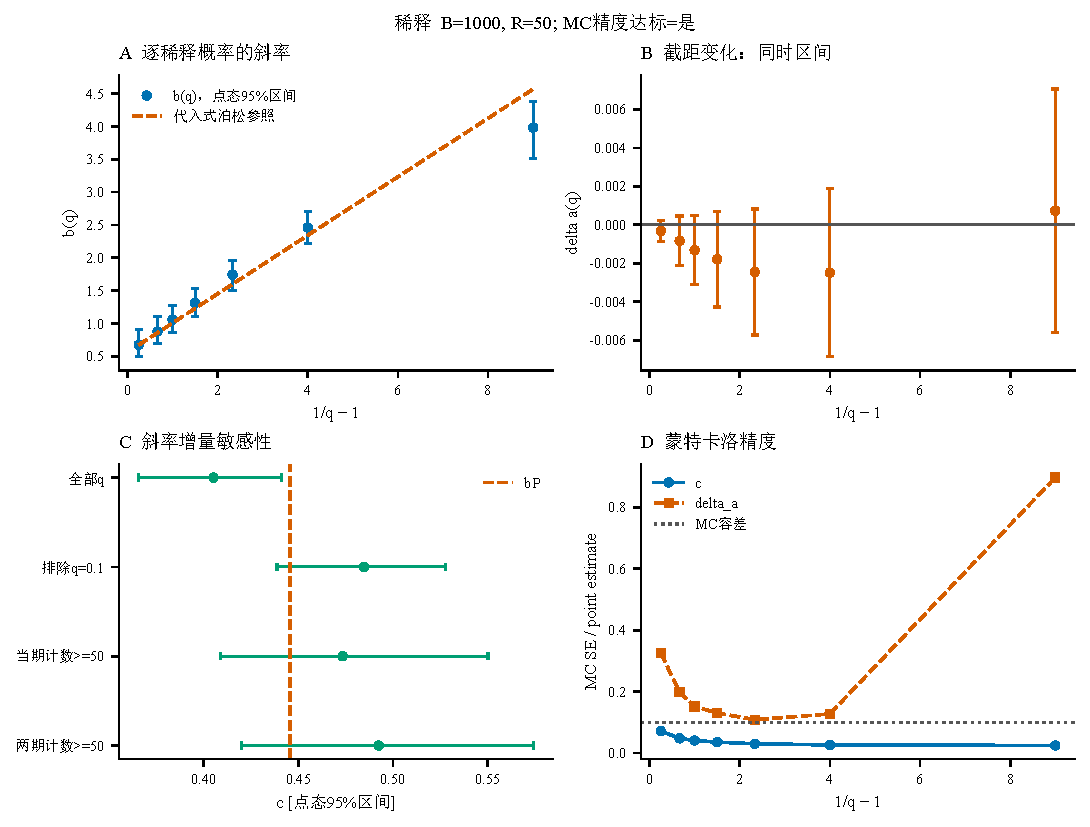
\includegraphics[width=\linewidth]{figures/fig_03_thinning.pdf}
\caption{固定样本上的受控稀释。重新计算统计量和中心后，在原始病例尺度上拟合系数。截距差区间带考虑不同保留率间的联合自助变异。敏感性包括全部水平、剔除 $q=0.1$，以及限制原始当前和下一周计数。泊松弹性系数是近似参照，不是所有非线性拟合系数的精确预测。实际内外层重复次数见表~\ref{tab:thinning}。}
\label{fig:thinning}
\end{figure}

\subsection{州异质性与损失参照选择}
\label{sec:res-fe}

对同一样本（$R_A$，n=\Nra{}），包含州截距和共同州内斜率时，$b_{\rm w}=\FEbPoint{}$（\FEbInterval{}），州截距均值为 \FEaPoint{}（\FEaInterval{}）。均值口径的比值为 \FEratioPoint{}（\FEratioInterval{}）；采用实际加权 $D_t$ 得到 \FEDratioPoint{}（\FEDratioInterval{}；图~\ref{fig:heterogeneity}、表~\ref{tab:fe}）。后一规格是独立拟合，不再是单周计数分析的别名。

独立重抽样日历周时，合并对州内的配对比值为 \FEpairedPoint{}（\FEpairedInterval{}）。两周、三周块区间分别为 \FEpairedBlockTwoInterval{} 和 \FEpairedBlockThreeInterval{}。普通区间下界略高于 1，时间块区间则包含 1。因此差异依赖于如何表示时间相关，不能转换为空间汇总的因果贡献比例。主州模型在 \FEBootstrap{} 次自助样本中有 \FEvalid{} 次有效拟合，有限有效重复区间的条件性及诊断失败均已标注。州与周双向点诊断未达到数值收敛标准，不报告斜率或置信区间。

改变损失参照同样会改变截距（表~\ref{tab:centering}）。保持共同全局归一化分母，用全国周中心替代合并中心后，$R_A$ 截距减少 \RAweekReductionPoint{}\%（\RAweekReductionInterval{}\%），$G$ 减少 \GweekReductionPoint{}\%（\GweekReductionInterval{}\%）。该降幅仅针对固定归一化分母；若同时改变归一化，将定义另一个不可直接比较的量。按季中心化与共同线性去趋势并不产生相同变化。不同参照移除不同的观测轨迹成分，其中包含真实共同信号。排除自身州的变体进一步记录一个观测参与自身周参照的影响。这些比较刻画定义敏感性，不构成独立传播与报告方差的已识别分解。

\begin{figure}[tbp]
\centering
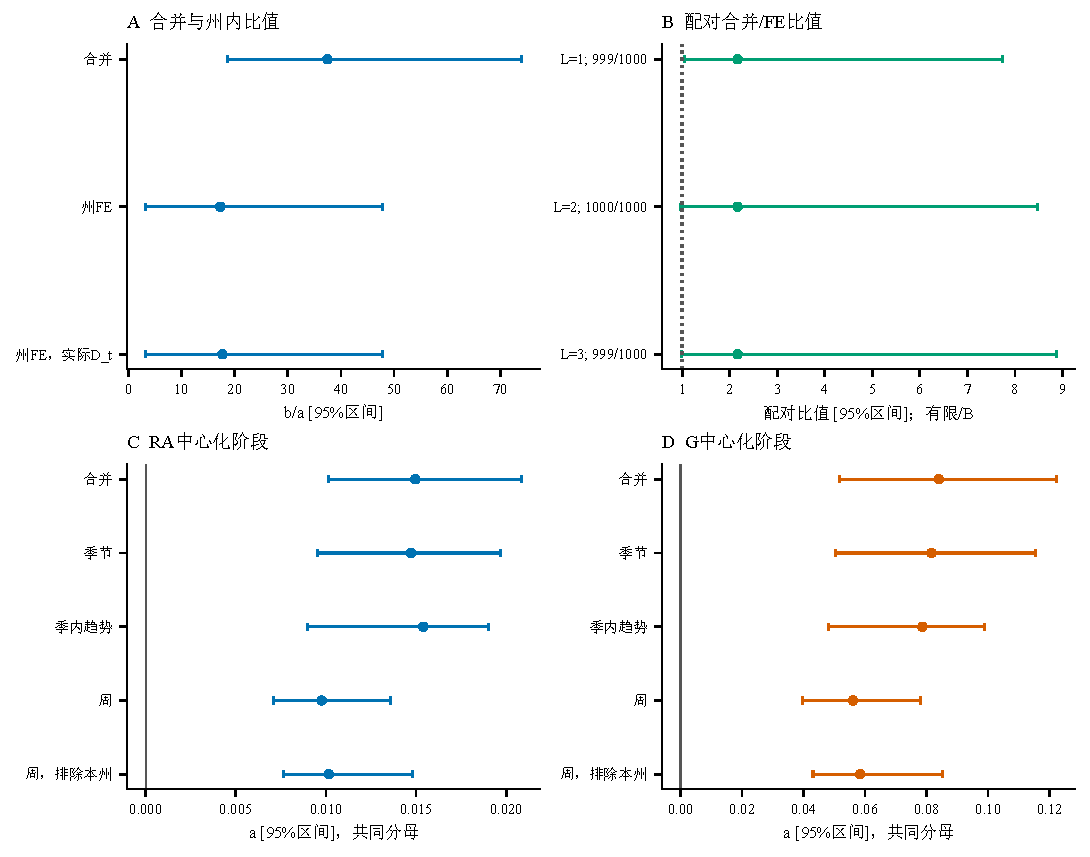
\includegraphics[width=\linewidth]{figures/fig_04_heterogeneity.pdf}
\caption{空间规格与参照敏感性。合并和州截距估计使用相同的全局损失定义；$D_t$ 敏感性使用加权滞后计数。参照调整保持全局归一化不变，仅改变中心或共同趋势。时间块配对区间展示对时间依赖处理的敏感性。未定义或未收敛结果不绘制成有效估计；不同参照对应不同经验目标。}
\label{fig:heterogeneity}
\end{figure}

\subsection{条件校准的限制}
\label{sec:res-sim}

补充校准对两种表观统计量使用修正后的观察机制，报告全部声明情景（表~\ref{tab:calibration}）。其中区分来源匹配的 3.2 天、标准差 2.1 天间隔，固定变异系数敏感性，以及历史 3.6 天代理。条件区间合并配对经验与模拟器不确定性，不对假造的间隔假设分布取平均。

模拟器可以重现截距，却不能同时重现斜率或有效样本量。因此响应检查保留这些差异，不通过抬高初始零计数或选择有利情景消除它们。初始条件和无输入感染的假设可使初始为零的州之后仍无感染，这不同于持续存在输入的现实监测。全国与州持续性、计数过度离散、报告波动在模拟器中也是不同机制；多个摘要相容并不能唯一识别其中一个。本文不据校准值断言有固定比例的真实州周超过生物学或经济门槛。

\section{讨论}
\label{sec:discussion}

理论结果是在明确观测模型下区分推断目标。报告固定已知、暴露规模外生且计数误差条件独立时，当期值风险为 $A/m$，已观测时期实现均值的风险为 $A/(Tm)$。估计平稳过程均值，还需计入该实现均值的方差。在固定时期内增加病例不会改变这一贡献，而随时期数增加时它如何变化取决于时间协方差。报告波动则会改变当期值与实现均值的风险。这些恒等式为解释病例量提供参照，其假设决定参照的适用范围。

这一方差结构在种群统计随机性、环境随机性与整群抽样中已有先例\citep{engen1998demographic, cochran1977sampling}。其监测含义取决于哪些量共同变化，以及估计意在描述什么。独立后代与独立报告产生随暴露规模下降的抽样误差；共同传播条件通过所抽取的时期影响过程均值估计；共同报告波动影响对这些时期的测量。把所有持续存在的分量都称为环境底线，会掩盖这一区别，并可能把目标本身的变异误当作测量误差。

条件信息计算与流行曲线信息量的分析相互补充\citep{parag2022quantifying, parag2022fundamental}。它确立了分母和报告分布已知时，尺度化计数在指定无偏估计量类中的有效性，并未确立再生数推断的普适下界。追加观测、独立报告测量与先验结构都会改变可用信息。以条件偏差换取较低方差的方法同样位于该估计量类之外。因此，平衡规模应始终附属于其估计量、目标与抽样实验，而不能视为病原体固有的属性。

另一个相关区别涉及估计窗口。在 Cori 框架中，扩大窗口可以累积感染压力与发病数，同时要求再生数在更长区间内局部恒定\citep{cori2013new, gostic2020practical}。这在时间分辨率与精度之间进行权衡，传播发生变化时可能引入模型失配。它不等同于抽取更多独立传播时期，也不会自动保持估计对象不变。表~\ref{tab:targets} 的重复时期平均使用另一种假设：每个时期各有其传播值，并有对该值条件无偏的测量。把这些公式用于重叠窗口时，需明确处理窗口重叠与时间相依性。

实证分析考察的是表观周统计量的相对偏差平方，而非相对于已观测 $R_t$ 的均方误差。第~\ref{sec:res-empirical}~节的仿射与幂律比较，涉及观测计数范围内得到支持的曲线形态。仅有正的拟合截距不能确立非零渐近极限，预测表现接近也不能识别生成任一曲线的机制。仅用训练样本确定中心与评分权重，可避免预测比较中的信息泄漏。前瞻曲线区分分析仍以其生成机制为条件，回答的问题不同于识别生物学传播方差。

受控稀释对已记录计数施加已知抽样操作。随机移除前的原始观测轨迹得到保留，但非线性变换、连续性校正与随机分母都可能改变两个拟合系数。基于导数的参照是对整个计算流程的近似，并非统计量的精确不变量。因此，解读第~\ref{sec:res-thinning}~节时，必须同时考虑各保留率下的响应、不确定性与已知计数模型检查。与参照响应一致，可以支持该局部抽样描述，却不能验证住院数据满足完整的 $A/m$ 恒等式，也不能识别未稀释斜率的来源。未拒绝截距变化不构成等效性的证据。

州截距拟合与替代中心方案回答不同的问题。州截距允许各州基准损失不同，同时估计损失与州内计数变化的关联；它不会使这种变化成为外生变量，也不会消除共同周冲击。重抽样摘要必须对应目标州分布，并计入抽中次数；未抽中的州没有已估计截距。按流行季、趋势或全国周重新中心化，改变了被建模的损失。相应截距变化是敏感性指标，并非正交的生物学方差分量。全国周均值的任何方差比，针对的是方法中定义的有符号偏差，而不会自动对应平方损失响应。

空间与时间相依性也约束不确定性。同周地区受到共同影响，同一地区的重复观测具有共同历史。交叉重抽样在其自身假设下处理这两类相依性\citep{owen2007pigeonhole, cameron2011robust}，限定于季内的时间块敏感性分析则考察剩余序列相依。无论增加同一流行季内的数据行，还是增加住院数，都不会提供独立流行季。类似地，如式~(\ref{eq:pooling}) 所示，空间聚合可以通过局部流行之间的协方差改变传播本身的变异。因此，横截面计数关联可能同时包含抽样精度与被平均人群差异的影响。

模拟反演以传播和观测机制为条件（第~\ref{sec:meth-inversion}~节与第~\ref{sec:res-sim}~节）。每日更新模拟器中指定的周再生数变异，是按日历周索引的模型参数，并非直接观测到的逐代真值；对病例数乘以时间换算因子，也不能换算其方差或平衡规模。独立观测离散、共同报告冲击与传播持续性必须分别规定。由同一住院序列计算的统计量彼此一致，是有用的一致性检查，但共同数据与共同校准假设限制了它作为证据的独立性。

代际间隔进一步限定这一映射。序列间隔、内禀代际间隔与家庭内实现代际间隔衡量不同的量\citep{cowling2009estimation, vink2014serial, chan2025estimating}。采用假定变异系数构造的敏感性分布，必须与来源研究报告的离散程度区分；间隔均值的置信限也不定义整个代际间隔分布的后验。条件校准区间与指定情景之间的变化描述不同的不确定性，情景范围不是联合置信区间。传播不确定性需要有依据的分布与明确的联合模型，不能靠给敏感性端点重新命名来实现。

最后，机构参与度只衡量检出过程的一方面。参与报告的医院内部，检测、就医、编码与入院实践也可能变化。缺乏识别政策效应的设计时，报告制度间比较仍属描述性分析。对这些过程的独立测量、更细空间观测以及更多流行季，可以直接应对主要识别限制。附录~\ref{app:extensions} 的符号化设计扩展示范所选目标如何进入资源分配，同时受成本、可行时期数和相依性约束。实际决策要求在一致尺度上测量这些量。单凭经验摘要，无法给出普适病例门槛或唯一识别的传播方差。

\section{结论}
\label{sec:conclusion}

病例量对于不同推断目标具有不同的统计价值。报告固定已知且暴露规模外生时，当期再生数与已观测时期实现均值的计数误差都会下降。估计平稳过程均值，还需抽样传播水平各异的时期，剩余不确定性取决于相依性。不可观测的报告波动即使对实现目标也贡献误差，计数矩一般无法将其与传播变异分离。表观周住院统计量衡量围绕所选中心的偏差，而非相对于已知传播真值的误差。曲线比较、稀释、州截距拟合与条件校准分别处理这一观测问题的一部分，不能识别普适病例门槛。在用病例量量化精度或分配资源之前，监测设计应先明确目标、观测机制与时间尺度。

\section*{数据与代码可用性声明}
\label{sec:availability}

NHSN 每周呼吸道住院数据可由美国疾病控制与预防中心公开获取\citep{cdc2026nhsn}；分析使用 2026-10-20 检索的快照。分析代码、固定分析窗口、模拟设定、版本化结果包与验证日志可在 \url{https://github.com/wangchi2068/reproduction-number-targets-surveillance} 获取。发布清单记录每个原始输入及生成资产的 SHA-256。本研究未使用个体级或受限数据。

\FloatBarrier
\bibliographystyle{elsarticle-harv}
\bibliography{bibliography}
\FloatBarrier
\clearpage
\appendix
\counterwithin{equation}{section}
\renewcommand{\theequation}{\thesection.\arabic{equation}}

\section{证明}
\label{app:proofs}

\subsection{计数分布与条件信息}
\label{app:model}
\label{app:target1}

单个负二项后代计数的概率生成函数为 $[1+(R_t/k)(1-z)]^{-k}$。条件独立使总后代的生成函数等于该函数的 $n$ 次幂。独立报告对应替换 $z\mapsto1-\rho+\rho z$，得到 $[1+(\rho R_t/k)(1-z)]^{-nk}$，从而证明式~(\ref{eq:observed})。对生成函数求导即得所列各矩。

对于固定已知的 $(n,\rho,k)$ 和 $R>0$，计数似然的得分与 Fisher 信息为
\begin{equation}
 \dot\ell(R)=\frac{c}{R}-\frac{(c+nk)\rho}{k+\rho R}
 =\mathcal I(R)(\Rhat-R),\qquad
 \mathcal I(R)=\frac{m}{R+\rho R^2/k}.
 \label{eq:score}
\end{equation}
因此 $\Var(\Rhat\mid R)=\mathcal I(R)^{-1}$。分布支持集不依赖于 $R$，正规的单参数 Cram\'er--Rao 不等式适用于对每个 $R$ 都无偏的估计量，给出第~\ref{sec:background}~节达到的下界\citep{lehmann1998theory}。这一计算不确立不受限制的决策理论下界，也不确立干扰参数未知时的下界。

\subsection{命题~\ref{prop:average} 的证明}
\label{app:prop1}

令 $e_t=\Rhat_t-R_t$，则 $\E(e_t\mid R_t)=0$，且
\begin{equation}
 \E(e_t^2)=\frac{\E R_t+\rho\E R_t^2/k}{m}=\frac{A}{m},
 \qquad \E[e_t(R_t-\Rbar)]=0.
\end{equation}
将式~(\ref{eq:error-split}) 平方即得式~(\ref{eq:var-average})。对基于同一计数且对每个 $R_t$ 条件无偏的任一估计量，其条件方差的期望至少为 $\E[\mathcal I(R_t)^{-1}]=A/m$，过程均值风险再加上相同的 $v_R$，由此证明限定估计量类中的最优性。固定 $\rho$、$k$ 与传播分布时，
\begin{equation}
 \frac{V(m)-V(2m)}{V(m)}=\frac{1}{2(1+m/\mx)},\qquad v_R>0.
\end{equation}
这一比较改变的是暴露规模 $n$；改变报告概率时，不能原样使用。

\subsection{推论~\ref{cor:targets} 的证明}
\label{app:cor-targets}

给定完整轨迹 $R_{1:T}$，各期 $e_t$ 独立且均值为零，因此两两不相关，并与轨迹的任何平方可积函数正交。于是
\begin{equation}
 \E\!\left[\left(T^{-1}\sum_t e_t\right)^2\right]=\frac{A}{Tm},\qquad
 \Var(\widehat{\Rbar}_T)=\Var(\Rbar_T)+\frac{A}{Tm}.
\end{equation}
若 $R_t$ 独立同分布，则 $\Var(\Rbar_T)=v_R/T$。在所述平稳自协方差条件下，对全部协方差对求和给出
$T^2\Var(\Rbar_T)=v_R[T+2\sum_{h=1}^{T-1}(T-h)\phi^h]$。
有限几何级数求和得到式~(\ref{eq:ar-sum})，包括 $T=1$ 与 $\phi=0$ 的情形\citep{hamilton1994time}。类似地，对空间协方差对求和得到式~(\ref{eq:pooling})，其中相关矩阵必须有效。

\subsection{命题~\ref{prop:report-noise} 与推论~\ref{cor:report-current} 的证明}
\label{app:prop2}
\label{app:cor-report-current}

记 $z_t=p_t/\rho$、$u_t=C_t/m-z_tR_t$。给定 $(R_t,p_t)$，$u_t$ 的均值为零。由 $p_t$ 与 $R_t$ 独立、$\E z_t=1$、$\E z_t^2=1+\tau^2$，有
\begin{equation}
 \E(u_t^2)=\frac{\Rbar+\rho(1+\tau^2)(\Rbar^2+v_R)/k}{m}
 =\frac{A_H}{m}.
\end{equation}
误差 $\Rhat_t-R_t=u_t+(z_t-1)R_t$ 的两项不相关，第二项的期望平方为 $\tau^2(\Rbar^2+v_R)=v_H$，从而证明式~(\ref{eq:vH-current})。又因 $\E(\Rhat_t-R_t\mid R_t)=0$，过程均值风险加上 $v_R$。在推论~\ref{cor:report-current} 的附加跨期假设下，给定传播轨迹并对报告积分后，这些误差独立且均值为零，故得式~(\ref{eq:report-means})。

对于识别结论，令 $U=(1+\tau^2)(\Rbar^2+v_R)$。尺度化计数的两个可观测矩满足
\begin{equation}
 \E\Rhat_t=\Rbar,\qquad
 \Var(\Rhat_t)=U-\Rbar^2+\frac{\Rbar+\rho U/k}{m}.
 \label{eq:moment-identification}
\end{equation}
只要不同且可行的 $\tau^2$ 给出 $v_R=U/(1+\tau^2)-\Rbar^2\ge0$，这些矩便相同。非退化边界以外存在这样的不同参数对，改变外生 $m$ 也不能将它们分离；同时仍须满足 $p_t$ 和 $R_t$ 的约束。由此证明基于这些矩的不可识别性，而不主张完整计数分布相同。

当 $v_R>0$ 时，广义平衡规模 $m_{\times,H}=A_H/(v_R+v_H)$ 满足
\begin{equation}
 \mx-m_{\times,H}
 =\frac{\tau^2(\Rbar^2+v_R)\Rbar(1+\rho\Rbar/k)}{v_R(v_R+v_H)}\ge0.
 \label{eq:mx-gap}
\end{equation}
对于 $\Rbar>0$，等号恰在 $\tau=0$ 时成立。这里较低的平衡规模伴随较高风险，并不意味着监测更准确。

\section{符号化理论扩展}
\label{app:extensions}

\subsection{预测与收缩估计}
\label{app:forecast}
\label{app:shrinkage}

在报告固定已知且满足推论~\ref{cor:targets} 的平稳协方差模型下，假定给定完整传播轨迹时，第 $t$ 期计数误差的均值为零，则
\begin{equation}
 \E[(\Rhat_t-R_{t+1})^2]=\frac{A}{m}+2(1-\phi)v_R.
\end{equation}
当 $\Rbar$、$v_R$ 和 $\phi$ 已知时，在形如 $\Rbar+\lambda(\Rhat_t-\Rbar)$ 的预测中最小化风险，得到
\begin{equation}
 \lambda^*=\frac{\phi v_R}{v_R+A/m},\qquad
 \mathrm{MSE}_{\mathrm{lin}}=v_R-\frac{\phi^2v_R^2}{v_R+A/m}.
 \label{eq:forecast}
\end{equation}
将风险展开为 $\lambda$ 的二次式并使用 $\Cov(\Rhat_t,R_{t+1})=\phi v_R$ 即得上述结果。其极限为 $(1-\phi^2)v_R$；传播时期独立时，该类中的最优预测为已知过程均值。最优性仅限于基于单个当期估计的线性预测，不涵盖全部历史或非线性预测量。

若改为估计 $\Rbar$，考虑 $\hat\theta_\lambda=(1-\lambda)\Rhat_t+\lambda\mu_0$，其中 $\mu_0$ 为固定基准、$\Delta=\mu_0-\Rbar$，其风险为
\begin{equation}
 \E[(\hat\theta_\lambda-\Rbar)^2]=(1-\lambda)^2V+\lambda^2\Delta^2,
 \qquad V=v_R+A/m.
\end{equation}
理想权重 $\lambda^*=V/(V+\Delta^2)$ 给出风险 $V\Delta^2/(V+\Delta^2)$，可能低于 $v_R$，说明无偏性限制的重要性。理想权重使用未知量；估计权重后需另行分析其风险。

\subsection{时期数可行约束下的预算分配}
\label{app:allocation}

\begin{proposition}[预算分配的连续松弛]
\label{prop:allocation}
\label{app:prop3}
在 H1--H4、传播时期独立同分布、计数条件独立、$\rho$ 固定及线性成本下，设 $\mathcal B=T(c_0+c_1m)$，其中 $c_0,c_1>0$。将 $T\ge1$ 与 $m>0$ 视为连续变量。当 $v_R>0$、$\mathcal B>c_0$ 时，无约束驻点为
\begin{equation}
 m^*=\sqrt{\frac{c_0A}{c_1v_R}}=\sqrt{\frac{c_0}{c_1}\mx}.
 \label{eq:optimal-m}
\end{equation}
可行最优解为 $\min\{m^*,(\mathcal B-c_0)/c_1\}$，再由预算约束恢复 $T$。若另有下限 $m_{\min}>0$，则在区间 $[m_{\min},(\mathcal B-c_0)/c_1]$ 非空时，将 $m^*$ 截取至该区间。
\end{proposition}

\begin{proof}
对独立同分布时期，过程均值风险为
\begin{equation}
 \frac{v_R}{T}+\frac{A}{Tm}
 =\frac{(c_0+c_1m)(v_R+A/m)}{\mathcal B}=:f(m).
 \label{eq:alloc-indep}
\end{equation}
其导数为 $f'(m)=(c_1v_R-c_0A/m^2)/\mathcal B$ 和 $f''(m)=2c_0A/(\mathcal B m^3)>0$。严格凸性给出驻点及截取后的解。当 $v_R=0$ 时，风险随 $m$ 下降，因此最优解是最大的可行 $m$；若无其他限制，对应 $T=1$。
\end{proof}

连续松弛具有熟悉的群规模分配形式\citep{cochran1977sampling, raudenbush1997statistical}。实际设计要求 $T$ 与 $n$ 为整数，且 $m=\rho n$。在预算不等式下，对每个可行整数 $T$，取
\begin{equation}
 n_T=\left\lfloor\frac{\mathcal B/T-c_0}{c_1\rho}\right\rfloor\ge1,
 \qquad m_T=\rho n_T,
\end{equation}
并在全部可行 $T$ 之间比较风险。这处理了预算剩余与 $T=1$ 的边界；仅对连续最优点取整未必足够。

\subsection{时间相依下的预算分配}
\label{app:budget-ar}

对平稳自协方差模型，应改为比较精确的整数设计目标函数
\begin{equation}
 F(T)=\frac{v_RS(\phi,T)}{T^2}+\frac{A}{Tm_T}.
 \label{eq:budget-ar-exact}
\end{equation}
该式不推出独立时期的最优解，也不推出普适切换门槛。若报告冲击独立，将其中计数项替换为 $(v_H+A_H/m_T)/T$。所有成本与暴露量必须对应同一时期；这些符号公式不能直接将周住院比值换算为代际设计门槛。

\subsection{覆盖规模与报告完整度}
\label{app:coverage}

固定传播分布，设可微的报告波动关系 $\tau^2(\rho)$ 不依赖于 $n$，记 $Q=\Rbar^2+v_R$。在 $\rho$ 的内点处，按比例增加 $n$ 与 $\rho$ 所带来的单期过程均值风险降幅分别为
\begin{equation}
\begin{aligned}
 -\frac{\partial V_H}{\partial\log n}
 &=\frac{\Rbar}{\rho n}+\frac{(1+\tau^2)Q}{kn},\\
 -\frac{\partial V_H}{\partial\log\rho}
 &=\frac{\Rbar}{\rho n}-\rho\frac{\mathrm d\tau^2}{\mathrm d\rho}\,Q\left(1+\frac{1}{kn}\right).
\end{aligned}
 \label{eq:coverage-gains}
\end{equation}
在代入 $m=\rho n$ 之前，对式~(\ref{eq:vH-AH}) 求导即得。固定 $\tau$ 时，第一项收益较大；若提高完整度同时稳定报告，这一次序可以改变。此处比较的是同比例变化，未按成本调整。

\begin{corollary}[指定的报告机制]
\label{cor:switch}
若 $p_t$ 是 $\nu$ 个独立报告单元中以概率 $\rho$ 参与者的比例，即 $\tau^2=(1-\rho)/(\rho\nu)$，则提高完整度的同比例收益更大，当且仅当
\begin{equation}
 m>\frac{\rho^2(\nu-1)}{k}.
 \label{eq:r3-switch}
\end{equation}
若 $p_t\sim\mathrm{Beta}(\rho\nu,(1-\rho)\nu)$，对应条件为 $m>\rho^2\nu/k$。
\end{corollary}

在报告单元模型中，第二个导数收益减去第一个为 $Q(kn)^{-1}[(kn+\rho)/(\rho\nu)-1]$。将 $\nu$ 替换为 $\nu+1$ 即证明 beta 情形。仅凭观测到的机构参与度，不能推出任一机制成立。

\subsection{条件更新矩与含噪分母}
\label{app:renewal}
\label{app:random-denominator}

可以明确陈述一个受限的更新模型类比。给定历史 $\mathcal F$，假定感染压力 $\Lambda>0$ 与下一期 $R$ 独立，且 $\E(R\mid\mathcal F)=\Rbar$、$\Var(R\mid\mathcal F)=v_R$。假定条件计数分布的均值为 $\rho\Lambda R$、方差为 $\rho\Lambda R+\rho^2\Lambda R^2/k$。令 $\bar\Lambda=\E(\Lambda\mid\mathcal F)$、$m=\rho\bar\Lambda$，全方差公式给出
\begin{equation}
 \frac{\Var(C\mid\mathcal F)}{m^2}
 =v_R+\frac{A}{m}
   +\frac{\Var(\Lambda\mid\mathcal F)}{\bar\Lambda^2}(\Rbar^2+v_R).
 \label{eq:renewal-conditional}
\end{equation}
该结果依赖刚刚陈述的条件独立与固定矩假设。它是计数预测方差，并非分母经估计的比值所满足的一般误差恒等式，也不解决发病数的内生性。

为说明比值问题，以正的潜在轨迹为条件，将分子和分母写为各自潜在值分别乘以 $(1+\varepsilon)$ 和 $(1+u)$。令 $Y=y(1+\varepsilon)/(1+u)$，其中扰动均值为零、阶为 $\tau$，分母远离零，尺度化三阶矩有界，且 Taylor 余项可积，则
\begin{equation}
\begin{aligned}
 \E(Y\mid y,\text{path})/y
 &=1+\E(u^2\mid\text{path})-\E(\varepsilon u\mid\text{path})+O(\tau^3),\\
 \Var(Y\mid\text{path})/y^2
 &=\Var(\varepsilon-u\mid\text{path})+O(\tau^3).
\end{aligned}
\end{equation}
分子与分母的协方差及诱导偏差都会进入表观变异。重叠比值可以共享扰动。这些条件近似不能给出拟合损失截距的精确来源分解。

\subsection{重复观测与方差估计}
\label{app:vr-precision}
\label{app:seasons}

\begin{proposition}[过程方差的条件信息下界]
\label{prop:vr-precision}
设 $R_1,\ldots,R_T$ 为独立同分布的伽马变量，已知均值为 $\Rbar$、方差为 $v_R>0$。若给定 $R_{1:T}$ 的观测分布不再以其他方式依赖于 $v_R$，则基于计数的任一正规无偏 $v_R$ 估计量，其相对标准误至少为
\begin{equation}
 [T\xi(\xi\psi'(\xi)-1)]^{-1/2},\qquad \xi=\Rbar^2/v_R,
 \label{eq:vr-bound}
\end{equation}
其中 $\psi'$ 为三伽马函数。
\end{proposition}

观测潜在 $R_t$ 所提供的信息，不可能少于仅观测由它们生成的计数。均值固定时，每期关于伽马形状参数 $\xi$ 的信息为 $\psi'(\xi)-1/\xi$；使用参数变换 $\mathrm d\xi/\mathrm dv_R=-\xi/v_R$ 即得下界。当 $\xi\to\infty$ 时，下界趋于 $\sqrt{2/T}$。

\begin{corollary}[独立流行季效应]
\label{cor:season}
设 $S\ge2$ 个流行季效应为独立同分布的高斯变量，均值未知、方差为 $v_S>0$，且其条件计数分布不含这些参数。对所有均值与方差均无偏的任一 $v_S$ 估计量，其相对标准误至少为 $\sqrt{2/(S-1)}$。
\end{corollary}

以潜在效应为条件取期望不能增加方差。其样本方差是一致最小方差无偏估计量，方差为 $2v_S^2/(S-1)$\citep{lehmann1998theory, searle1992variance}。因此，对于该下界，增加已有流行季内的观测不能替代独立流行季。两种下界都是有条件的模型结果，并非经验置信限。

\FloatBarrier
\clearpage
\renewcommand{\thetable}{S\arabic{table}}
\setcounter{table}{0}
\renewcommand{\thefigure}{S\arabic{figure}}
\setcounter{figure}{0}
\section{补充方法与结果}
\label{app:supplement}

\subsection{输入登记与可复现性}
\label{app:inputs}

全部报告结果均由发布清单记录 SHA-256 的 NHSN 原始州周表重建。面板将缺失值保持为缺失，并要求四个连续周日期，不插入零住院。主样本与全部固定窗口由发布版中的确定性键标识。所有保留的表格、图件和正文数值宏均由同一版本化结果包生成；清单记录输入哈希、生成器哈希、实际自助预算、拟合失败与蒙特卡洛诊断。续跑必须匹配完整的源码、输入与配置指纹，否则重新运行。

表~\ref{tab:pooled} 报告合并仿射工作拟合及三种代际间隔变换。3.6 天与固定变异系数设定均明确列为选择；3.2 天、标准差 2.1 天设定复现 \citet{chan2025estimating} 的内禀间隔估计。表~\ref{tab:cv} 报告仅用训练折中心和拟合的逐折留出评分。季节折使用与拟合相同的数据，属描述性结果。

校准登记表将每个输入标明为有据外部估计、由观测面板导出或分析假设。延迟、后代离散度、住院概率与周冲击方差在模拟器中是假设，其作用是结构敏感性而非测量。观察模型以二项住院分配为基准；$\varphi>1$ 表示直接从潜在强度生成、条件方差为 $\varphi\lambda$ 的伽马--泊松计数。模拟器检查条件观察矩与直接计数构造；这些检验验证实现，不证明经验适用性。

\subsection{条件校准}
\label{app:calibration}

每个声明情景在四个固定观测窗口长度和观测首周州计数上模拟。初始零计数保持为零，不抬高；这可能使保留样本小于实证面板，差异在响应诊断中保留。周再生数冲击区分全国与州分量；报告持续性属于另一机制。再生数新息在声明的正下界处截断，并记录截断比例。

对每个实证统计量，用加权直线联系模拟平均截距与声明周方差网格。配对经验抽样与配对模拟面板共同形成条件反演抽样。拟合失败、非有限值、非正隐含值与网格外推均计数并报告；百分位区间只针对有限抽样，并标注条件性。多个情景可给出相近实证摘要而观察机制不同。因此校准报告截距、斜率、样本量、有符号偏差方差比及州内与全国滞后一阶自相关的响应检查，不指定唯一生物学方差或某机制正确的概率。

\subsection{次要敏感性与设计示例}
\label{app:secondary}

表~\ref{tab:secondary} 报告分季截距，以及将各统计量计数除以机构参与率、同时保留原尺度的配对调整。该调整只测记录到的参与率代理；报告机构内部的检测强度、编码与就诊行为未观测。三个夏季摘要未经调整，仅描述单次自愿报告期，不是因果比较或独立重复。本文不声称等效性或报告制度效应。

表~\ref{tab:design} 报告模型条件下的曲线辨别示例。观测季节设计按声明计数倍率循环，并叠加均值为一的交叉对数正态变异；生成曲线为拟合的仿射与幂律均值。校准分位与评价模拟相互独立；在解释功效前先报告零假设拒绝比例及精确二项区间。所有单元的功效都接近 1。这种饱和说明合成生成机制远比真实数据有利，而真实数据中两条曲线无法区分；因此该练习不能回答现实需要多少季节，仅用于记录这一局限。附录~\ref{app:allocation} 的预算表达式保持符号形式；不将周住院比转换为代际设计门槛。

\begin{table}[htbp]
\centering
\small
\caption{合并仿射损失拟合与代际间隔敏感性}\label{tab:pooled}
\setlength{\tabcolsep}{2pt}
\begin{tabularx}{\linewidth}{@{}>{\raggedright\arraybackslash}p{0.2400\linewidth}>{\raggedright\arraybackslash}p{0.1750\linewidth}>{\raggedright\arraybackslash}p{0.1750\linewidth}>{\raggedright\arraybackslash}p{0.1750\linewidth}>{\raggedright\arraybackslash}p{0.1750\linewidth}@{}}
\toprule
统计量 & 参数 & n & 估计值 [95\% CI] & 有限/B \\
\midrule
RA & a & 1748 & 0.01495 [0.01001, 0.02092] & 2000/2000 \\
RA & b & 1748 & 0.56 [0.369, 0.7692] & 2000/2000 \\
RA & b/a & 1748 & 37.44 [18.93, 69.92] & 2000/2000 \\
G & a & 1756 & 0.08401 [0.04986, 0.1234] & 2000/2000 \\
G & b & 1756 & 1.971 [0.9889, 3.042] & 2000/2000 \\
G & b/a & 1756 & 23.46 [8.279, 54.7] & 2000/2000 \\
RA32 & a & 1748 & 0.01191 [0.007997, 0.01668] & 2000/2000 \\
RA32 & b & 1748 & 0.4482 [0.2975, 0.6147] & 2000/2000 \\
RA32 & b/a & 1748 & 37.62 [19.13, 69.89] & 2000/2000 \\
RA32source & a & 1748 & 0.01106 [0.007501, 0.01553] & 2000/2000 \\
RA32source & b & 1748 & 0.4196 [0.2827, 0.5688] & 2000/2000 \\
RA32source & b/a & 1748 & 37.93 [19.42, 69.26] & 2000/2000 \\
\bottomrule
\end{tabularx}
\par\smallskip
\begin{minipage}{\linewidth}\footnotesize\raggedright
有符号百分位区间；比值只在分母为正时定义。逐项保留有限重抽样次数。 RA a: 2000/2000 有限重抽样; RA b: 2000/2000 有限重抽样; RA ratio: 2000/2000 有限重抽样; G a: 2000/2000 有限重抽样; G b: 2000/2000 有限重抽样; G ratio: 2000/2000 有限重抽样; RA32 a: 2000/2000 有限重抽样; RA32 b: 2000/2000 有限重抽样; RA32 ratio: 2000/2000 有限重抽样; RA32source a: 2000/2000 有限重抽样; RA32source b: 2000/2000 有限重抽样; RA32source ratio: 2000/2000 有限重抽样.
\end{minipage}
\end{table}

\begin{table}[htbp]
\centering
\scriptsize
\caption{逐折模型验证}\label{tab:cv}
\setlength{\tabcolsep}{2pt}
\begin{tabularx}{\linewidth}{@{}>{\raggedright\arraybackslash}p{0.2400\linewidth}>{\raggedright\arraybackslash}p{0.1167\linewidth}>{\raggedright\arraybackslash}p{0.1167\linewidth}>{\raggedright\arraybackslash}p{0.1167\linewidth}>{\raggedright\arraybackslash}p{0.1167\linewidth}>{\raggedright\arraybackslash}p{0.1167\linewidth}>{\raggedright\arraybackslash}p{0.1167\linewidth}@{}}
\toprule
统计量/划分 & 折 & 有效/总数或n & 仿射 & 幂律 & 差值 & 胜出/有效 \\
\midrule
RA / 州 & 汇总 & 51/51 & -- & -- & -0.002018 & 26 \\
RA / 季 & 汇总 & 4/4 & -- & -- & 0.004626 & 3 \\
RA & 2022-23 & 365 & -2.378 & -2.369 & 0.008954 & 是 \\
RA & 2023-24 & 499 & -2.613 & -2.612 & 0.0008806 & 是 \\
RA & 2024-25 & 356 & -2.46 & -2.481 & -0.02077 & 是 \\
RA & 2025-26 & 528 & -2.346 & -2.324 & 0.0223 & 是 \\
G / 州 & 汇总 & 51/51 & -- & -- & -0.007369 & 22 \\
G / 季 & 汇总 & 4/4 & -- & -- & -0.004414 & 2 \\
G & 2022-23 & 367 & -0.5979 & -0.5942 & 0.003756 & 是 \\
G & 2023-24 & 503 & -1.201 & -1.192 & 0.008487 & 是 \\
G & 2024-25 & 357 & -0.7333 & -0.7584 & -0.02505 & 是 \\
G & 2025-26 & 529 & -0.7557 & -0.7641 & -0.008421 & 是 \\
RA32 / 州 & 汇总 & 51/51 & -- & -- & -0.002242 & 25 \\
RA32 / 季 & 汇总 & 4/4 & -- & -- & 0.004343 & 3 \\
RA32 & 2022-23 & 365 & -2.612 & -2.604 & 0.00805 & 是 \\
RA32 & 2023-24 & 499 & -2.83 & -2.83 & 0.0001619 & 是 \\
RA32 & 2024-25 & 356 & -2.691 & -2.712 & -0.02118 & 是 \\
RA32 & 2025-26 & 528 & -2.572 & -2.549 & 0.02294 & 是 \\
RA32source / 州 & 汇总 & 51/51 & -- & -- & -0.002824 & 25 \\
RA32source / 季 & 汇总 & 4/4 & -- & -- & 0.003577 & 2 \\
RA32source & 2022-23 & 365 & -2.701 & -2.695 & 0.005641 & 是 \\
RA32source & 2023-24 & 499 & -2.886 & -2.888 & -0.001735 & 是 \\
RA32source & 2024-25 & 356 & -2.77 & -2.792 & -0.02217 & 是 \\
RA32source & 2025-26 & 528 & -2.644 & -2.619 & 0.02453 & 是 \\
\bottomrule
\end{tabularx}
\par\smallskip
\begin{minipage}{\linewidth}\footnotesize\raggedright
汇总行列出有效/总折数及末列偏向仿射模型的折数；季节行列出测试样本量与收敛状态。评分为平均 L/mu + log(mu)，越低越好。差值=幂律减仿射，正值偏向仿射。各折重新拟合训练中心。训练集重叠，不报告独立折标准误或四季显著性检验。
\end{minipage}
\end{table}

\begin{table}[htbp]
\centering
\scriptsize
\caption{共享计数稀释估计、同时区间与模拟诊断}\label{tab:thinning}
\setlength{\tabcolsep}{2pt}
\begin{tabularx}{\linewidth}{@{}>{\raggedright\arraybackslash}p{0.2400\linewidth}>{\raggedright\arraybackslash}p{0.1400\linewidth}>{\raggedright\arraybackslash}p{0.1400\linewidth}>{\raggedright\arraybackslash}p{0.1400\linewidth}>{\raggedright\arraybackslash}p{0.1400\linewidth}>{\raggedright\arraybackslash}p{0.1400\linewidth}@{}}
\toprule
样本 & q/拟合 & 指标 & 估计值 [95\% CI] & 同时95\%区间 & 有限/B \\
\midrule
full & q=0.8 & b & 0.6747 [0.4905, 0.9034] & -- & 1000/1000 \\
full & q=0.8 & c & 0.4588 [0.3731, 0.5557] & [0.3381, 0.5795] & 1000/1000 \\
full & q=0.8 & delta\_\allowbreak{}a & -0.0003183 [-0.000786, 0.00005128] & [-0.0008833, 0.0002467] & 1000/1000 \\
full & q=0.8 & c\_\allowbreak{}over\_\allowbreak{}bP & 1.03 [0.8476, 1.242] & -- & 1000/1000 \\
full & q=0.6 & b & 0.8763 [0.6941, 1.103] & -- & 1000/1000 \\
full & q=0.6 & c & 0.4745 [0.4064, 0.5532] & [0.3751, 0.574] & 1000/1000 \\
full & q=0.6 & delta\_\allowbreak{}a & -0.000836 [-0.001963, -0.000006555] & [-0.00213, 0.0004583] & 1000/1000 \\
full & q=0.6 & c\_\allowbreak{}over\_\allowbreak{}bP & 1.065 [0.915, 1.241] & -- & 1000/1000 \\
full & q=0.5 & b & 1.057 [0.858, 1.275] & -- & 1000/1000 \\
full & q=0.5 & c & 0.4969 [0.4243, 0.5606] & [0.4047, 0.589] & 1000/1000 \\
full & q=0.5 & delta\_\allowbreak{}a & -0.001318 [-0.002744, -0.00009326] & [-0.003126, 0.0004903] & 1000/1000 \\
full & q=0.5 & c\_\allowbreak{}over\_\allowbreak{}bP & 1.115 [0.9621, 1.252] & -- & 1000/1000 \\
full & q=0.4 & b & 1.31 [1.112, 1.534] & -- & 1000/1000 \\
full & q=0.4 & c & 0.4997 [0.4397, 0.5611] & [0.4158, 0.5837] & 1000/1000 \\
full & q=0.4 & delta\_\allowbreak{}a & -0.001794 [-0.00376, -0.0001502] & [-0.004272, 0.0006837] & 1000/1000 \\
full & q=0.4 & c\_\allowbreak{}over\_\allowbreak{}bP & 1.122 [0.9903, 1.257] & -- & 1000/1000 \\
full & q=0.3 & b & 1.742 [1.503, 1.958] & -- & 1000/1000 \\
full & q=0.3 & c & 0.5067 [0.4482, 0.5539] & [0.4326, 0.5808] & 1000/1000 \\
full & q=0.3 & delta\_\allowbreak{}a & -0.002454 [-0.004852, -0.000159] & [-0.005728, 0.0008198] & 1000/1000 \\
full & q=0.3 & c\_\allowbreak{}over\_\allowbreak{}bP & 1.137 [1.008, 1.249] & -- & 1000/1000 \\
full & q=0.2 & b & 2.46 [2.221, 2.711] & -- & 1000/1000 \\
full & q=0.2 & c & 0.4749 [0.4292, 0.5229] & [0.4126, 0.5373] & 1000/1000 \\
full & q=0.2 & delta\_\allowbreak{}a & -0.002484 [-0.005751, 0.0005387] & [-0.006867, 0.001899] & 1000/1000 \\
full & q=0.2 & c\_\allowbreak{}over\_\allowbreak{}bP & 1.066 [0.9728, 1.173] & -- & 1000/1000 \\
full & q=0.1 & b & 3.983 [3.509, 4.379] & -- & 1000/1000 \\
full & q=0.1 & c & 0.3804 [0.3337, 0.4204] & [0.3234, 0.4373] & 1000/1000 \\
full & q=0.1 & delta\_\allowbreak{}a & 0.0007312 [-0.00305, 0.005984] & [-0.005595, 0.007057] & 1000/1000 \\
full & q=0.1 & c\_\allowbreak{}over\_\allowbreak{}bP & 0.8537 [0.7415, 0.9566] & -- & 1000/1000 \\
full & full & c & 0.4051 [0.3656, 0.4413] & -- & 1000/1000 \\
full & full & c\_\allowbreak{}over\_\allowbreak{}bP & 0.9093 [0.8101, 0.9995] & -- & 1000/1000 \\
full & full & delta\_\allowbreak{}a\_\allowbreak{}rate & -0.0001293 [-0.0006192, 0.0004699] & -- & 1000/1000 \\
full & noq01 & c & 0.4848 [0.4387, 0.5279] & -- & 1000/1000 \\
full & noq01 & c\_\allowbreak{}over\_\allowbreak{}bP & 1.088 [0.9936, 1.186] & -- & 1000/1000 \\
full & noq01 & delta\_\allowbreak{}a\_\allowbreak{}rate & -0.0008058 [-0.001703, 0.00005179] & -- & 1000/1000 \\
highCt50 & q=0.8 & b & 0.7797 [-0.007567, 1.573] & -- & 1000/1000 \\
highCt50 & q=0.8 & c & 0.442 [0.2771, 0.6691] & [0.1838, 0.7002] & 1000/1000 \\
highCt50 & q=0.8 & delta\_\allowbreak{}a & -0.00007119 [-0.0004223, 0.0001553] & [-0.0004703, 0.0003279] & 1000/1000 \\
highCt50 & q=0.8 & c\_\allowbreak{}over\_\allowbreak{}bP & 1.051 [0.6634, 1.606] & -- & 1000/1000 \\
highCt50 & q=0.6 & b & 0.969 [0.1971, 1.773] & -- & 1000/1000 \\
highCt50 & q=0.6 & c & 0.4497 [0.3339, 0.6318] & [0.256, 0.6433] & 1000/1000 \\
highCt50 & q=0.6 & delta\_\allowbreak{}a & -0.0001877 [-0.0009664, 0.0002652] & [-0.0009926, 0.0006171] & 1000/1000 \\
highCt50 & q=0.6 & c\_\allowbreak{}over\_\allowbreak{}bP & 1.069 [0.8015, 1.51] & -- & 1000/1000 \\
highCt50 & q=0.5 & b & 1.126 [0.3593, 1.891] & -- & 1000/1000 \\
highCt50 & q=0.5 & c & 0.4567 [0.3405, 0.6213] & [0.273, 0.6404] & 1000/1000 \\
highCt50 & q=0.5 & delta\_\allowbreak{}a & -0.0002913 [-0.001459, 0.0003529] & [-0.001456, 0.000873] & 1000/1000 \\
highCt50 & q=0.5 & c\_\allowbreak{}over\_\allowbreak{}bP & 1.086 [0.8187, 1.476] & -- & 1000/1000 \\
highCt50 & q=0.4 & b & 1.351 [0.6322, 2.134] & -- & 1000/1000 \\
highCt50 & q=0.4 & c & 0.4548 [0.3568, 0.593] & [0.2972, 0.6124] & 1000/1000 \\
highCt50 & q=0.4 & delta\_\allowbreak{}a & -0.0004078 [-0.001854, 0.0004131] & [-0.001938, 0.001122] & 1000/1000 \\
highCt50 & q=0.4 & c\_\allowbreak{}over\_\allowbreak{}bP & 1.081 [0.8483, 1.413] & -- & 1000/1000 \\
highCt50 & q=0.3 & b & 1.723 [1.005, 2.495] & -- & 1000/1000 \\
highCt50 & q=0.3 & c & 0.4515 [0.3668, 0.5711] & [0.3176, 0.5854] & 1000/1000 \\
highCt50 & q=0.3 & delta\_\allowbreak{}a & -0.0005649 [-0.00247, 0.0006027] & [-0.002578, 0.001448] & 1000/1000 \\
highCt50 & q=0.3 & c\_\allowbreak{}over\_\allowbreak{}bP & 1.073 [0.8687, 1.355] & -- & 1000/1000 \\
highCt50 & q=0.2 & b & 2.522 [1.77, 3.276] & -- & 1000/1000 \\
highCt50 & q=0.2 & c & 0.4633 [0.3813, 0.5611] & [0.3435, 0.5831] & 1000/1000 \\
highCt50 & q=0.2 & delta\_\allowbreak{}a & -0.0009427 [-0.00351, 0.0008025] & [-0.003822, 0.001937] & 1000/1000 \\
highCt50 & q=0.2 & c\_\allowbreak{}over\_\allowbreak{}bP & 1.102 [0.9074, 1.325] & -- & 1000/1000 \\
highCt50 & q=0.1 & b & 4.97 [4.216, 5.814] & -- & 999/1000 \\
highCt50 & q=0.1 & c & 0.4778 [0.4127, 0.5552] & [0.3835, 0.5721] & 999/1000 \\
highCt50 & q=0.1 & delta\_\allowbreak{}a & -0.001594 [-0.005615, 0.001213] & [-0.006149, 0.002962] & 999/1000 \\
highCt50 & q=0.1 & c\_\allowbreak{}over\_\allowbreak{}bP & 1.136 [0.9843, 1.323] & -- & 999/1000 \\
highCt50 & full & c & 0.4734 [0.409, 0.5503] & -- & 999/1000 \\
highCt50 & full & c\_\allowbreak{}over\_\allowbreak{}bP & 1.126 [0.9702, 1.316] & -- & 999/1000 \\
highCt50 & full & delta\_\allowbreak{}a\_\allowbreak{}rate & -0.0001928 [-0.0006891, 0.0001441] & -- & 999/1000 \\
highCt50 & noq01 & c & 0.4594 [0.3808, 0.5603] & -- & 1000/1000 \\
highCt50 & noq01 & c\_\allowbreak{}over\_\allowbreak{}bP & 1.092 [0.9026, 1.327] & -- & 1000/1000 \\
highCt50 & noq01 & delta\_\allowbreak{}a\_\allowbreak{}rate & -0.0002434 [-0.0009563, 0.0002083] & -- & 1000/1000 \\
both50 & q=0.8 & b & 0.5473 [-0.2021, 1.391] & -- & 1000/1000 \\
both50 & q=0.8 & c & 0.4994 [0.3073, 0.7827] & [0.1979, 0.8009] & 1000/1000 \\
both50 & q=0.8 & delta\_\allowbreak{}a & -0.0001674 [-0.0006684, 0.0001096] & [-0.0006864, 0.0003517] & 1000/1000 \\
both50 & q=0.8 & c\_\allowbreak{}over\_\allowbreak{}bP & 1.194 [0.722, 1.896] & -- & 1000/1000 \\
both50 & q=0.6 & b & 0.754 [0.02843, 1.586] & -- & 1000/1000 \\
both50 & q=0.6 & c & 0.4973 [0.3582, 0.7249] & [0.2629, 0.7317] & 1000/1000 \\
both50 & q=0.6 & delta\_\allowbreak{}a & -0.0004007 [-0.001555, 0.000186] & [-0.001503, 0.0007021] & 1000/1000 \\
both50 & q=0.6 & c\_\allowbreak{}over\_\allowbreak{}bP & 1.189 [0.854, 1.751] & -- & 1000/1000 \\
both50 & q=0.5 & b & 0.9288 [0.1947, 1.748] & -- & 1000/1000 \\
both50 & q=0.5 & c & 0.5063 [0.3635, 0.7058] & [0.2897, 0.723] & 1000/1000 \\
both50 & q=0.5 & delta\_\allowbreak{}a & -0.0006083 [-0.00219, 0.0001859] & [-0.002149, 0.0009326] & 1000/1000 \\
both50 & q=0.5 & c\_\allowbreak{}over\_\allowbreak{}bP & 1.21 [0.8863, 1.69] & -- & 1000/1000 \\
both50 & q=0.4 & b & 1.161 [0.4133, 1.977] & -- & 1000/1000 \\
both50 & q=0.4 & c & 0.4921 [0.3785, 0.6457] & [0.3095, 0.6746] & 1000/1000 \\
both50 & q=0.4 & delta\_\allowbreak{}a & -0.00078 [-0.002694, 0.0002525] & [-0.002738, 0.001178] & 1000/1000 \\
both50 & q=0.4 & c\_\allowbreak{}over\_\allowbreak{}bP & 1.176 [0.9064, 1.548] & -- & 1000/1000 \\
both50 & q=0.3 & b & 1.554 [0.8611, 2.363] & -- & 1000/1000 \\
both50 & q=0.3 & c & 0.4849 [0.3882, 0.6214] & [0.3325, 0.6373] & 1000/1000 \\
both50 & q=0.3 & delta\_\allowbreak{}a & -0.001058 [-0.003465, 0.0003471] & [-0.003573, 0.001457] & 1000/1000 \\
both50 & q=0.3 & c\_\allowbreak{}over\_\allowbreak{}bP & 1.159 [0.9271, 1.485] & -- & 1000/1000 \\
both50 & q=0.2 & b & 2.382 [1.63, 3.167] & -- & 1000/1000 \\
both50 & q=0.2 & c & 0.4899 [0.3955, 0.5995] & [0.3589, 0.6209] & 1000/1000 \\
both50 & q=0.2 & delta\_\allowbreak{}a & -0.001588 [-0.004831, 0.0005575] & [-0.005049, 0.001874] & 1000/1000 \\
both50 & q=0.2 & c\_\allowbreak{}over\_\allowbreak{}bP & 1.171 [0.9456, 1.432] & -- & 1000/1000 \\
both50 & q=0.1 & b & 4.863 [4.1, 5.734] & -- & 999/1000 \\
both50 & q=0.1 & c & 0.4934 [0.4221, 0.5729] & [0.3956, 0.5913] & 999/1000 \\
both50 & q=0.1 & delta\_\allowbreak{}a & -0.002397 [-0.007015, 0.000824] & [-0.007548, 0.002755] & 999/1000 \\
both50 & q=0.1 & c\_\allowbreak{}over\_\allowbreak{}bP & 1.18 [1.005, 1.371] & -- & 999/1000 \\
both50 & full & c & 0.4926 [0.42, 0.5742] & -- & 999/1000 \\
both50 & full & c\_\allowbreak{}over\_\allowbreak{}bP & 1.178 [1.004, 1.379] & -- & 999/1000 \\
both50 & full & delta\_\allowbreak{}a\_\allowbreak{}rate & -0.0003058 [-0.000896, 0.00009878] & -- & 999/1000 \\
both50 & noq01 & c & 0.4898 [0.3971, 0.6072] & -- & 1000/1000 \\
both50 & noq01 & c\_\allowbreak{}over\_\allowbreak{}bP & 1.171 [0.9533, 1.462] & -- & 1000/1000 \\
both50 & noq01 & delta\_\allowbreak{}a\_\allowbreak{}rate & -0.0004328 [-0.001331, 0.0001204] & -- & 1000/1000 \\
\bottomrule
\end{tabularx}
\par\smallskip
\begin{minipage}{\linewidth}\footnotesize\raggedright
逐q区间为点态区间；单列包络为各子集中跨q的同时区间。full使用全部q；noq01排除q=0.1。highCt50要求原当期计数>=50；both50要求原相邻两期计数均>=50。c为每(1/q-1)的斜率增量；bP为代入式泊松参照。 B=1000; R(point)=400; R(inner, actual)=50; precision criterion: MC SE at most 0.1 times the point estimate, applied to the five monitored response summaries; max finite MC SE/|point| over all stored metrics=68.44; max finite MC SE/sampling SE over all stored metrics=1.74; undefined MC ratios=0/219; MC status=tolerance\_\allowbreak{}met. Point fits 8400/8400; bootstrap fits 1049998/1050000; failed bootstrap averages=2. Any failed inner fit makes that q average undefined; no silent averaging over successful fits. full: n=1748; bP=0.4455 [0.4282, 0.4658]. highCt50: n=828; bP=0.4206 [0.4032, 0.4387]. both50: n=821; bP=0.4183 [0.4008, 0.4359].
\end{minipage}
\end{table}

\begin{table}[htbp]
\centering
\scriptsize
\caption{R\_\allowbreak{}A 样本（n=1748）的固定效应：配对比值、周块敏感性与收敛}\label{tab:fe}
\setlength{\tabcolsep}{2pt}
\begin{tabularx}{\linewidth}{@{}>{\raggedright\arraybackslash}p{0.2400\linewidth}>{\raggedright\arraybackslash}p{0.1750\linewidth}>{\raggedright\arraybackslash}p{0.1750\linewidth}>{\raggedright\arraybackslash}p{0.1750\linewidth}>{\raggedright\arraybackslash}p{0.1750\linewidth}@{}}
\toprule
周块 & 参数 & 估计值 [95\% CI] & 有限/B & 非正比例/诊断 \\
\midrule
L=1 & Pooled a & 0.01495 [0.009976, 0.02114] & 1000/1000 & 0 \\
L=1 & Pooled b & 0.56 [0.3682, 0.7707] & 1000/1000 & 0 \\
L=1 & Pooled b/a & 37.44 [18.64, 73.92] & 1000/1000 & 0 \\
L=1 & State FE b & 0.3794 [0.1082, 0.6403] & 999/1000 & 0 \\
L=1 & State FE mean a & 0.02192 [0.01289, 0.03502] & 999/1000 & 0 \\
L=1 & State FE b/mean a & 17.3 [3.315, 47.8] & 999/1000 & 0 \\
L=1 & State FE median a & 0.01751 [0.01037, 0.03014] & 999/1000 & 0 \\
L=1 & State FE b/median a & 21.67 [3.977, 57.85] & 999/1000 & 0 \\
L=1 & State FE row-weighted a & 0.02061 [0.01339, 0.03114] & 999/1000 & 0 \\
L=1 & State FE row-weighted ratio & 18.41 [3.705, 45.56] & 999/1000 & 0 \\
L=1 & State FE count-weighted a & 0.01542 [0.01056, 0.02288] & 999/1000 & 0 \\
L=1 & State FE count-weighted ratio & 24.61 [5.265, 55.65] & 999/1000 & 0 \\
L=1 & True D\_\allowbreak{}t b & 0.3691 [0.1153, 0.6145] & 999/1000 & 0 \\
L=1 & True D\_\allowbreak{}t mean a & 0.02084 [0.01218, 0.03429] & 999/1000 & 0 \\
L=1 & True D\_\allowbreak{}t ratio & 17.71 [3.267, 47.81] & 999/1000 & 0 \\
L=1 & Paired pooled/FE ratio & 2.164 [1.04, 7.745] & 999/1000 & 0 \\
L=2 & Pooled a & 0.01495 [0.009493, 0.02077] & 1000/1000 & 0 \\
L=2 & Pooled b & 0.56 [0.371, 0.763] & 1000/1000 & 0 \\
L=2 & Pooled b/a & 37.44 [18.73, 74.77] & 1000/1000 & 0 \\
L=2 & State FE b & 0.3794 [0.109, 0.6611] & 1000/1000 & 0 \\
L=2 & State FE mean a & 0.02192 [0.01288, 0.03581] & 1000/1000 & 0 \\
L=2 & State FE b/mean a & 17.3 [3.453, 50.16] & 1000/1000 & 0 \\
L=2 & State FE median a & 0.01751 [0.01024, 0.03013] & 1000/1000 & 0 \\
L=2 & State FE b/median a & 21.67 [3.984, 60.15] & 1000/1000 & 0 \\
L=2 & State FE row-weighted a & 0.02061 [0.013, 0.03107] & 1000/1000 & 0 \\
L=2 & State FE row-weighted ratio & 18.41 [3.819, 48.17] & 1000/1000 & 0 \\
L=2 & State FE count-weighted a & 0.01542 [0.0102, 0.02293] & 1000/1000 & 0 \\
L=2 & State FE count-weighted ratio & 24.61 [5.111, 57.08] & 1000/1000 & 0 \\
L=2 & True D\_\allowbreak{}t b & 0.3691 [0.1082, 0.612] & 1000/1000 & 0.001 \\
L=2 & True D\_\allowbreak{}t mean a & 0.02084 [0.01168, 0.03555] & 1000/1000 & 0 \\
L=2 & True D\_\allowbreak{}t ratio & 17.71 [3.26, 51.13] & 1000/1000 & 0.001 \\
L=2 & Paired pooled/FE ratio & 2.164 [0.964, 8.483] & 1000/1000 & 0 \\
L=3 & Pooled a & 0.01495 [0.01001, 0.02089] & 1000/1000 & 0 \\
L=3 & Pooled b & 0.56 [0.3851, 0.7603] & 1000/1000 & 0 \\
L=3 & Pooled b/a & 37.44 [19.39, 68.59] & 1000/1000 & 0 \\
L=3 & State FE b & 0.3794 [0.111, 0.6669] & 1000/1000 & 0.001 \\
L=3 & State FE mean a & 0.02192 [0.01247, 0.03692] & 1000/1000 & 0 \\
L=3 & State FE b/mean a & 17.3 [3.051, 50.11] & 1000/1000 & 0.001 \\
L=3 & State FE median a & 0.01751 [0.01068, 0.03045] & 1000/1000 & 0 \\
L=3 & State FE b/median a & 21.67 [3.982, 58.24] & 1000/1000 & 0.001 \\
L=3 & State FE row-weighted a & 0.02061 [0.01293, 0.0317] & 1000/1000 & 0 \\
L=3 & State FE row-weighted ratio & 18.41 [3.407, 47.65] & 1000/1000 & 0.001 \\
L=3 & State FE count-weighted a & 0.01542 [0.01076, 0.02338] & 1000/1000 & 0 \\
L=3 & State FE count-weighted ratio & 24.61 [4.841, 57.62] & 1000/1000 & 0.001 \\
L=3 & True D\_\allowbreak{}t b & 0.3691 [0.1072, 0.6252] & 1000/1000 & 0.001 \\
L=3 & True D\_\allowbreak{}t mean a & 0.02084 [0.0116, 0.03629] & 1000/1000 & 0 \\
L=3 & True D\_\allowbreak{}t ratio & 17.71 [3.068, 51.41] & 1000/1000 & 0.001 \\
L=3 & Paired pooled/FE ratio & 2.164 [0.9866, 8.87] & 999/1000 & 0 \\
点估计诊断 & week\_\allowbreak{}only & b=0.5258 & 无区间 & group\_\allowbreak{}gamma\_\allowbreak{}objective\_\allowbreak{}fallback \\
点估计诊断 & state\_\allowbreak{}and\_\allowbreak{}week & 不可用 & 无区间 & iteration\_\allowbreak{}limit \\
\bottomrule
\end{tabularx}
\par\smallskip
\begin{minipage}{\linewidth}\footnotesize\raggedright
样本为 \$R\_\allowbreak{}A\$ 规格的 1748 个州周、51 个辖区；本表不使用 \$G\$ 样本。区间保留有符号重抽样；有限/B<1时，区间以有限估计为条件。末列为全部请求重抽样中的非正比例。FE以抽中的州出现次数为目标；合并/FE比较在重抽样内配对。L为季内周块长度。仅周和州加周拟合为点估计诊断，失败时无估计或区间。本表合并行使用本表自身的 1000 次自助抽样，可能与表 S1 的 2000 次主区间略有差异。 L=1 pooled: 1000 converged, 0 failed; \{\}. L=1 state: 999 converged, 1 failed; \{"gamma\_\allowbreak{}objective\_\allowbreak{}fallback\_\allowbreak{}failed": 1\}. L=1 state\_\allowbreak{}D: 999 converged, 1 failed; \{"gamma\_\allowbreak{}objective\_\allowbreak{}fallback\_\allowbreak{}failed": 1\}. L=2 pooled: 1000 converged, 0 failed; \{\}. L=2 state: 1000 converged, 0 failed; \{\}. L=2 state\_\allowbreak{}D: 1000 converged, 0 failed; \{\}. L=3 pooled: 1000 converged, 0 failed; \{\}. L=3 state: 1000 converged, 0 failed; \{\}. L=3 state\_\allowbreak{}D: 1000 converged, 0 failed; \{\}.
\end{minipage}
\end{table}

\begin{table}[htbp]
\centering
\scriptsize
\caption{采用共同损失分母的中心化阶段}\label{tab:centering}
\setlength{\tabcolsep}{2pt}
\begin{tabularx}{\linewidth}{@{}>{\raggedright\arraybackslash}p{0.2400\linewidth}>{\raggedright\arraybackslash}p{0.1750\linewidth}>{\raggedright\arraybackslash}p{0.1750\linewidth}>{\raggedright\arraybackslash}p{0.1750\linewidth}>{\raggedright\arraybackslash}p{0.1750\linewidth}@{}}
\toprule
统计量/中心 & 合并均值 & a / 变化 [95\% CI] & b [95\% CI] & 有限/B \\
\midrule
RA / pooled & 1.206 & 0.01495 [0.01016, 0.02083] & 0.56 [0.3625, 0.7639] & 1000/1000 \\
RA / season & 1.206 & 0.01471 [0.009507, 0.01966] & 0.5391 [0.3602, 0.7205] & 1000/1000 \\
RA / season\_\allowbreak{}linear & 1.206 & 0.0154 [0.008972, 0.01901] & 0.3936 [0.2717, 0.5763] & 1000/1000 \\
RA / week & 1.206 & 0.009766 [0.007103, 0.01357] & 0.4581 [0.3124, 0.5916] & 1000/1000 \\
RA / week\_\allowbreak{}leave\_\allowbreak{}state\_\allowbreak{}out & 1.206 & 0.01016 [0.007654, 0.01481] & 0.4841 [0.3492, 0.6636] & 1000/1000 \\
RA / week\_\allowbreak{}change & 1.206 & -0.005189 [-0.01015, -0.0006938] & -- & 1000/1000 \\
RA / week\_\allowbreak{}reduction\_\allowbreak{}fraction & 1.206 & 34.7 [5.967, 51.9] & -- & 1000/1000 \\
G / pooled & 1.724 & 0.08401 [0.05163, 0.1222] & 1.971 [0.9987, 2.986] & 1000/1000 \\
G / season & 1.724 & 0.08163 [0.0504, 0.1156] & 1.842 [0.9591, 2.602] & 1000/1000 \\
G / season\_\allowbreak{}linear & 1.724 & 0.07864 [0.04808, 0.09897] & 1.249 [0.6423, 1.988] & 1000/1000 \\
G / week & 1.724 & 0.05607 [0.03962, 0.07812] & 1.401 [0.7134, 1.912] & 1000/1000 \\
G / week\_\allowbreak{}leave\_\allowbreak{}state\_\allowbreak{}out & 1.724 & 0.05843 [0.04308, 0.08505] & 1.477 [0.8089, 2.138] & 1000/1000 \\
G / week\_\allowbreak{}change & 1.724 & -0.02794 [-0.05687, -0.003708] & -- & 1000/1000 \\
G / week\_\allowbreak{}reduction\_\allowbreak{}fraction & 1.724 & 33.25 [6.805, 51.63] & -- & 1000/1000 \\
\bottomrule
\end{tabularx}
\par\smallskip
\begin{minipage}{\linewidth}\footnotesize\raggedright
同一统计量的五种中心均使用相同合并均值作为相对损失分母；每次重抽样用权重重新拟合该分母。week\_\allowbreak{}leave\_\allowbreak{}state\_\allowbreak{}out的周中心排除本州。减少比例为100*(a\_\allowbreak{}pooled-a\_\allowbreak{}week)/a\_\allowbreak{}pooled，单位为百分比；这些是描述性变化，并非可加总方差分量。本表区间使用自身的 1000 次自助抽样，可能与表 S1 的 2000 次主区间略有差异。 RA/pooled: 1000/1000 有限重抽样; RA/season: 1000/1000 有限重抽样; RA/season\_\allowbreak{}linear: 1000/1000 有限重抽样; RA/week: 1000/1000 有限重抽样; RA/week\_\allowbreak{}leave\_\allowbreak{}state\_\allowbreak{}out: 1000/1000 有限重抽样; G/pooled: 1000/1000 有限重抽样; G/season: 1000/1000 有限重抽样; G/season\_\allowbreak{}linear: 1000/1000 有限重抽样; G/week: 1000/1000 有限重抽样; G/week\_\allowbreak{}leave\_\allowbreak{}state\_\allowbreak{}out: 1000/1000 有限重抽样.
\end{minipage}
\end{table}

\begin{table}[htbp]
\centering
\scriptsize
\caption{全部声明情景的条件校准}\label{tab:calibration}
\setlength{\tabcolsep}{2pt}
\begin{tabularx}{\linewidth}{@{}>{\raggedright\arraybackslash}p{0.2400\linewidth}>{\raggedright\arraybackslash}p{0.1400\linewidth}>{\raggedright\arraybackslash}p{0.1400\linewidth}>{\raggedright\arraybackslash}p{0.1400\linewidth}>{\raggedright\arraybackslash}p{0.1400\linewidth}>{\raggedright\arraybackslash}p{0.1400\linewidth}@{}}
\toprule
情景/统计量 & v [95\% CI] & 有限/B & 非正/非有限 & 超网格/斜率<=0 & 失败拟合/全部 \\
\midrule
delay\_\allowbreak{}long / RA & 0.04587 [0.02996, 0.06461] & 2000/2000 & 0/0 & 0/0 & 0/1000 \\
delay\_\allowbreak{}long / G & 0.04686 [0.02666, 0.06952] & 2000/2000 & 0/0 & 3/0 & 0/1000 \\
delay\_\allowbreak{}short / RA & 0.03863 [0.02531, 0.05527] & 2000/2000 & 0/0 & 0/0 & 0/1000 \\
delay\_\allowbreak{}short / G & 0.04161 [0.02382, 0.06314] & 2000/2000 & 0/0 & 0/0 & 0/1000 \\
joint\_\allowbreak{}gi3.2\_\allowbreak{}pn0.25\_\allowbreak{}obs1 / RA & 0.02882 [0.01937, 0.04107] & 2000/2000 & 0/0 & 0/0 & 0/1000 \\
joint\_\allowbreak{}gi3.2\_\allowbreak{}pn0.25\_\allowbreak{}obs1 / G & 0.02967 [0.01709, 0.04456] & 2000/2000 & 0/0 & 0/0 & 0/1000 \\
joint\_\allowbreak{}gi3.2\_\allowbreak{}pn0.25\_\allowbreak{}obs1.25 / RA & 0.02844 [0.01853, 0.03995] & 2000/2000 & 0/0 & 0/0 & 0/1000 \\
joint\_\allowbreak{}gi3.2\_\allowbreak{}pn0.25\_\allowbreak{}obs1.25 / G & 0.0294 [0.01681, 0.04331] & 2000/2000 & 0/0 & 0/0 & 0/1000 \\
joint\_\allowbreak{}gi3.2\_\allowbreak{}pn0\_\allowbreak{}obs1 / RA & 0.03178 [0.02085, 0.04488] & 2000/2000 & 0/0 & 0/0 & 0/1000 \\
joint\_\allowbreak{}gi3.2\_\allowbreak{}pn0\_\allowbreak{}obs1 / G & 0.03369 [0.01924, 0.05045] & 2000/2000 & 0/0 & 0/0 & 0/1000 \\
joint\_\allowbreak{}gi3.2\_\allowbreak{}pn0\_\allowbreak{}obs1.25 / RA & 0.03128 [0.02019, 0.04538] & 2000/2000 & 0/0 & 0/0 & 0/1000 \\
joint\_\allowbreak{}gi3.2\_\allowbreak{}pn0\_\allowbreak{}obs1.25 / G & 0.03348 [0.01895, 0.05184] & 2000/2000 & 0/0 & 0/0 & 0/1000 \\
joint\_\allowbreak{}gi3.6\_\allowbreak{}pn0.25\_\allowbreak{}obs1 / RA & 0.03764 [0.02444, 0.05359] & 2000/2000 & 0/0 & 0/0 & 0/1000 \\
joint\_\allowbreak{}gi3.6\_\allowbreak{}pn0.25\_\allowbreak{}obs1 / G & 0.03902 [0.02247, 0.05689] & 2000/2000 & 0/0 & 0/0 & 0/1000 \\
joint\_\allowbreak{}gi3.6\_\allowbreak{}pn0.25\_\allowbreak{}obs1.25 / RA & 0.03638 [0.02354, 0.0519] & 2000/2000 & 0/0 & 0/0 & 0/1000 \\
joint\_\allowbreak{}gi3.6\_\allowbreak{}pn0.25\_\allowbreak{}obs1.25 / G & 0.03785 [0.0216, 0.05704] & 2000/2000 & 0/0 & 0/0 & 0/1000 \\
joint\_\allowbreak{}gi3.6\_\allowbreak{}pn0\_\allowbreak{}obs1 / RA & 0.04002 [0.02558, 0.05767] & 2000/2000 & 0/0 & 0/0 & 0/1000 \\
joint\_\allowbreak{}gi3.6\_\allowbreak{}pn0\_\allowbreak{}obs1 / G & 0.04282 [0.02407, 0.06368] & 2000/2000 & 0/0 & 0/0 & 0/1000 \\
joint\_\allowbreak{}gi3.6\_\allowbreak{}pn0\_\allowbreak{}obs1.25 / RA & 0.04035 [0.02648, 0.0569] & 2000/2000 & 0/0 & 0/0 & 0/1000 \\
joint\_\allowbreak{}gi3.6\_\allowbreak{}pn0\_\allowbreak{}obs1.25 / G & 0.04356 [0.02576, 0.064] & 2000/2000 & 0/0 & 0/0 & 0/1000 \\
k01 / RA & 0.04023 [0.02553, 0.05736] & 2000/2000 & 0/0 & 0/0 & 0/1000 \\
k01 / G & 0.04289 [0.02475, 0.0645] & 2000/2000 & 0/0 & 0/0 & 0/1000 \\
matched32\_\allowbreak{}binomial / RA & 0.03108 [0.02037, 0.04399] & 2000/2000 & 0/0 & 0/0 & 0/1000 \\
matched32\_\allowbreak{}binomial / G & 0.03287 [0.0186, 0.0489] & 2000/2000 & 0/0 & 0/0 & 0/1000 \\
matched32\_\allowbreak{}source\_\allowbreak{}sd21\_\allowbreak{}binomial / RA & 0.02884 [0.01908, 0.04027] & 2000/2000 & 0/0 & 0/0 & 0/1000 \\
matched32\_\allowbreak{}source\_\allowbreak{}sd21\_\allowbreak{}binomial / G & 0.031 [0.01794, 0.04533] & 2000/2000 & 0/0 & 0/0 & 0/1000 \\
matched36\_\allowbreak{}binomial / RA & 0.04 [0.02623, 0.0562] & 2000/2000 & 0/0 & 0/0 & 0/1000 \\
matched36\_\allowbreak{}binomial / G & 0.04298 [0.02466, 0.06284] & 2000/2000 & 0/0 & 0/0 & 0/1000 \\
national\_\allowbreak{}persistence25 / RA & 0.0369 [0.0238, 0.05109] & 2000/2000 & 0/0 & 0/0 & 0/1000 \\
national\_\allowbreak{}persistence25 / G & 0.03817 [0.02185, 0.05643] & 2000/2000 & 0/0 & 0/0 & 0/1000 \\
national\_\allowbreak{}share0 / RA & 0.03935 [0.0255, 0.05576] & 2000/2000 & 0/0 & 0/0 & 0/1000 \\
national\_\allowbreak{}share0 / G & 0.0416 [0.02393, 0.06162] & 2000/2000 & 0/0 & 0/0 & 0/1000 \\
national\_\allowbreak{}share65 / RA & 0.04014 [0.02576, 0.05685] & 2000/2000 & 0/0 & 0/0 & 0/1000 \\
national\_\allowbreak{}share65 / G & 0.04327 [0.02461, 0.06553] & 2000/2000 & 0/0 & 0/0 & 0/1000 \\
reporting\_\allowbreak{}shock / RA & 0.01954 [0.006213, 0.0358] & 2000/2000 & 0/0 & 0/0 & 0/1000 \\
reporting\_\allowbreak{}shock / G & 0.02903 [0.0117, 0.04918] & 2000/2000 & 0/0 & 0/0 & 0/1000 \\
rho\_\allowbreak{}h005 / RA & 0.03991 [0.02639, 0.05628] & 2000/2000 & 0/0 & 0/0 & 0/1000 \\
rho\_\allowbreak{}h005 / G & 0.04283 [0.02548, 0.06297] & 2000/2000 & 0/0 & 0/0 & 0/1000 \\
rho\_\allowbreak{}h02 / RA & 0.04029 [0.02632, 0.05694] & 2000/2000 & 0/0 & 0/0 & 0/1000 \\
rho\_\allowbreak{}h02 / G & 0.04317 [0.02494, 0.06466] & 2000/2000 & 0/0 & 0/0 & 0/1000 \\
state\_\allowbreak{}persistence50 / RA & 0.03244 [0.02095, 0.04559] & 2000/2000 & 0/0 & 0/0 & 0/1000 \\
state\_\allowbreak{}persistence50 / G & 0.03137 [0.01788, 0.0467] & 2000/2000 & 0/0 & 0/0 & 0/1000 \\
true2.2\_\allowbreak{}analyst36 / RA & 0.0146 [0.009442, 0.02045] & 2000/2000 & 0/0 & 0/0 & 0/1000 \\
true2.2\_\allowbreak{}analyst36 / G & 0.01473 [0.008358, 0.02141] & 2000/2000 & 0/0 & 0/0 & 0/1000 \\
true2.9\_\allowbreak{}analyst36 / RA & 0.02551 [0.0168, 0.03572] & 2000/2000 & 0/0 & 0/0 & 0/1000 \\
true2.9\_\allowbreak{}analyst36 / G & 0.02679 [0.01524, 0.0401] & 2000/2000 & 0/0 & 0/0 & 0/1000 \\
true4.3\_\allowbreak{}analyst36 / RA & 0.05807 [0.03763, 0.08382] & 2000/2000 & 0/0 & 27/0 & 0/1000 \\
true4.3\_\allowbreak{}analyst36 / G & 0.06312 [0.0366, 0.0955] & 2000/2000 & 0/0 & 78/0 & 0/1000 \\
\bottomrule
\end{tabularx}
\par\smallskip
\begin{minipage}{\linewidth}\footnotesize\raggedright
v为给定模型下、施加下界之前的周边际方差，不是已识别的生物学方差或上界。区间取全部有限有符号重抽样的2.5和97.5百分位；不作仅保留正值的筛选或截断。各列分别列出非正/非有限反演次数、超网格/非正斜率次数，以及失败/尝试的模拟拟合次数。 delay\_\allowbreak{}long: grid=[0.0, 0.02, 0.04, 0.06, 0.09]; RA point outside=False, nonpositive=False, max |line residual|/MC SE=0.8913; G point outside=False, nonpositive=False, max |line residual|/MC SE=0.5474. delay\_\allowbreak{}short: grid=[0.0, 0.02, 0.04, 0.06, 0.09]; RA point outside=False, nonpositive=False, max |line residual|/MC SE=1.781; G point outside=False, nonpositive=False, max |line residual|/MC SE=1.162. joint\_\allowbreak{}gi3.2\_\allowbreak{}pn0.25\_\allowbreak{}obs1: grid=[0.0, 0.02, 0.04, 0.06, 0.09]; RA point outside=False, nonpositive=False, max |line residual|/MC SE=0.974; G point outside=False, nonpositive=False, max |line residual|/MC SE=1.154. joint\_\allowbreak{}gi3.2\_\allowbreak{}pn0.25\_\allowbreak{}obs1.25: grid=[0.0, 0.02, 0.04, 0.06, 0.09]; RA point outside=False, nonpositive=False, max |line residual|/MC SE=1.557; G point outside=False, nonpositive=False, max |line residual|/MC SE=1.668. joint\_\allowbreak{}gi3.2\_\allowbreak{}pn0\_\allowbreak{}obs1: grid=[0.0, 0.02, 0.04, 0.06, 0.09]; RA point outside=False, nonpositive=False, max |line residual|/MC SE=1.13; G point outside=False, nonpositive=False, max |line residual|/MC SE=1.116. joint\_\allowbreak{}gi3.2\_\allowbreak{}pn0\_\allowbreak{}obs1.25: grid=[0.0, 0.02, 0.04, 0.06, 0.09]; RA point outside=False, nonpositive=False, max |line residual|/MC SE=1.369; G point outside=False, nonpositive=False, max |line residual|/MC SE=1.917. joint\_\allowbreak{}gi3.6\_\allowbreak{}pn0.25\_\allowbreak{}obs1: grid=[0.0, 0.02, 0.04, 0.06, 0.09]; RA point outside=False, nonpositive=False, max |line residual|/MC SE=1.666; G point outside=False, nonpositive=False, max |line residual|/MC SE=1.308. joint\_\allowbreak{}gi3.6\_\allowbreak{}pn0.25\_\allowbreak{}obs1.25: grid=[0.0, 0.02, 0.04, 0.06, 0.09]; RA point outside=False, nonpositive=False, max |line residual|/MC SE=1.255; G point outside=False, nonpositive=False, max |line residual|/MC SE=1.081. joint\_\allowbreak{}gi3.6\_\allowbreak{}pn0\_\allowbreak{}obs1: grid=[0.0, 0.02, 0.04, 0.06, 0.09]; RA point outside=False, nonpositive=False, max |line residual|/MC SE=1.596; G point outside=False, nonpositive=False, max |line residual|/MC SE=1.363. joint\_\allowbreak{}gi3.6\_\allowbreak{}pn0\_\allowbreak{}obs1.25: grid=[0.0, 0.02, 0.04, 0.06, 0.09]; RA point outside=False, nonpositive=False, max |line residual|/MC SE=0.9047; G point outside=False, nonpositive=False, max |line residual|/MC SE=0.9728. k01: grid=[0.0, 0.02, 0.04, 0.06, 0.09]; RA point outside=False, nonpositive=False, max |line residual|/MC SE=1.074; G point outside=False, nonpositive=False, max |line residual|/MC SE=1.429. matched32\_\allowbreak{}binomial: grid=[0.0, 0.02, 0.04, 0.06, 0.09]; RA point outside=False, nonpositive=False, max |line residual|/MC SE=0.4468; G point outside=False, nonpositive=False, max |line residual|/MC SE=0.4955. matched32\_\allowbreak{}source\_\allowbreak{}sd21\_\allowbreak{}binomial: grid=[0.0, 0.02, 0.04, 0.06, 0.09]; RA point outside=False, nonpositive=False, max |line residual|/MC SE=1.05; G point outside=False, nonpositive=False, max |line residual|/MC SE=0.9843. matched36\_\allowbreak{}binomial: grid=[0.0, 0.02, 0.04, 0.06, 0.09]; RA point outside=False, nonpositive=False, max |line residual|/MC SE=2.388; G point outside=False, nonpositive=False, max |line residual|/MC SE=1.795. national\_\allowbreak{}persistence25: grid=[0.0, 0.02, 0.04, 0.06, 0.09]; RA point outside=False, nonpositive=False, max |line residual|/MC SE=2.246; G point outside=False, nonpositive=False, max |line residual|/MC SE=2.37. national\_\allowbreak{}share0: grid=[0.0, 0.02, 0.04, 0.06, 0.09]; RA point outside=False, nonpositive=False, max |line residual|/MC SE=0.8455; G point outside=False, nonpositive=False, max |line residual|/MC SE=0.6427. national\_\allowbreak{}share65: grid=[0.0, 0.02, 0.04, 0.06, 0.09]; RA point outside=False, nonpositive=False, max |line residual|/MC SE=1.134; G point outside=False, nonpositive=False, max |line residual|/MC SE=0.7098. reporting\_\allowbreak{}shock: grid=[0.0, 0.02, 0.04, 0.06, 0.09]; RA point outside=False, nonpositive=False, max |line residual|/MC SE=0.8369; G point outside=False, nonpositive=False, max |line residual|/MC SE=0.9846. rho\_\allowbreak{}h005: grid=[0.0, 0.02, 0.04, 0.06, 0.09]; RA point outside=False, nonpositive=False, max |line residual|/MC SE=1.481; G point outside=False, nonpositive=False, max |line residual|/MC SE=1.628. rho\_\allowbreak{}h02: grid=[0.0, 0.02, 0.04, 0.06, 0.09]; RA point outside=False, nonpositive=False, max |line residual|/MC SE=1.184; G point outside=False, nonpositive=False, max |line residual|/MC SE=1.261. state\_\allowbreak{}persistence50: grid=[0.0, 0.02, 0.04, 0.06, 0.09]; RA point outside=False, nonpositive=False, max |line residual|/MC SE=3.259; G point outside=False, nonpositive=False, max |line residual|/MC SE=3.007. true2.2\_\allowbreak{}analyst36: grid=[0.0, 0.02, 0.04, 0.06, 0.09]; RA point outside=False, nonpositive=False, max |line residual|/MC SE=1.281; G point outside=False, nonpositive=False, max |line residual|/MC SE=1.023. true2.9\_\allowbreak{}analyst36: grid=[0.0, 0.02, 0.04, 0.06, 0.09]; RA point outside=False, nonpositive=False, max |line residual|/MC SE=0.5604; G point outside=False, nonpositive=False, max |line residual|/MC SE=1.366. true4.3\_\allowbreak{}analyst36: grid=[0.0, 0.02, 0.04, 0.06, 0.09]; RA point outside=False, nonpositive=False, max |line residual|/MC SE=1.162; G point outside=False, nonpositive=False, max |line residual|/MC SE=1.198.
\end{minipage}
\end{table}

\begin{table}[htbp]
\centering
\small
\caption{给定模型下的设计检验大小与功效}\label{tab:design}
\setlength{\tabcolsep}{2pt}
\begin{tabularx}{\linewidth}{@{}>{\raggedright\arraybackslash}p{0.2400\linewidth}>{\raggedright\arraybackslash}p{0.1400\linewidth}>{\raggedright\arraybackslash}p{0.1400\linewidth}>{\raggedright\arraybackslash}p{0.1400\linewidth}>{\raggedright\arraybackslash}p{0.1400\linewidth}>{\raggedright\arraybackslash}p{0.1400\linewidth}@{}}
\toprule
季数 & 计数倍数 & 大小 [95\% CI] & 功效 [95\% CI] & 有效C/N/A & 大小相容 \\
\midrule
4 & 1 & 0.058 [0.03918, 0.08224] & 0.996 [0.9856, 0.9995] & 500/500/500 & 是 \\
4 & 2 & 0.06 [0.04084, 0.08455] & 0.998 [0.9889, 0.9999] & 500/500/500 & 是 \\
4 & 4 & 0.052 [0.03425, 0.07527] & 0.994 [0.9826, 0.9988] & 500/500/500 & 是 \\
8 & 1 & 0.058 [0.03918, 0.08224] & 1 [0.9926, 1] & 500/500/500 & 是 \\
8 & 2 & 0.038 [0.02303, 0.05871] & 1 [0.9926, 1] & 500/500/500 & 是 \\
8 & 4 & 0.082 [0.05949, 0.1096] & 1 [0.9926, 1] & 500/500/500 & 否 \\
12 & 1 & 0.058 [0.03918, 0.08224] & 1 [0.9926, 1] & 500/500/500 & 是 \\
12 & 2 & 0.07 [0.04924, 0.09601] & 1 [0.9926, 1] & 500/500/500 & 是 \\
12 & 4 & 0.054 [0.03588, 0.0776] & 1 [0.9926, 1] & 500/500/500 & 是 \\
20 & 1 & 0.032 [0.0184, 0.05145] & 1 [0.9926, 1] & 500/500/500 & 是 \\
20 & 2 & 0.058 [0.03918, 0.08224] & 1 [0.9926, 1] & 500/500/500 & 是 \\
20 & 4 & 0.056 [0.03753, 0.07992] & 1 [0.9926, 1] & 500/500/500 & 是 \\
\bottomrule
\end{tabularx}
\par\smallskip
\begin{minipage}{\linewidth}\footnotesize\raggedright
条件区分模拟复用观测季节/计数设计，校准与评估样本独立。有效次数依次为校准/零假设/备择假设。末列表示检验大小区间是否包含名义alpha；保留全部单元，包括大小检验不通过的单元。这些模拟不意味着普适季节门槛或普适80\%功效。 alpha=0.05; replicates/stage=500.
\end{minipage}
\end{table}

\begin{table}[htbp]
\centering
\scriptsize
\caption{分季拟合与报告参与率敏感性}\label{tab:secondary}
\setlength{\tabcolsep}{2pt}
\begin{tabularx}{\linewidth}{@{}>{\raggedright\arraybackslash}p{0.2400\linewidth}>{\raggedright\arraybackslash}p{0.1400\linewidth}>{\raggedright\arraybackslash}p{0.1400\linewidth}>{\raggedright\arraybackslash}p{0.1400\linewidth}>{\raggedright\arraybackslash}p{0.1400\linewidth}>{\raggedright\arraybackslash}p{0.1400\linewidth}@{}}
\toprule
统计量/时期 & n & a / 变化 [95\% CI] & b / 原a & b/a / 调整a & 有限/B \\
\midrule
RA / 2022-23 & 365 & 0.01369 [0.0071, 0.02102] & 0.6967 & 50.91 & 1000/1000 \\
RA / 2023-24 & 499 & 0.006174 [0.002667, 0.01542] & 0.7018 & 113.7 & 1000/1000 \\
RA / 2024-25 & 356 & 0.01268 [0.005687, 0.02276] & 0.5826 & 45.93 & 1000/1000 \\
RA / 2025-26 & 528 & 0.02253 [0.008432, 0.03509] & 0.3533 & 15.68 & 1000/1000 \\
RA / 报告调整 & 1748 & 0.0002939 [-0.0003183, 0.0008476] & 0.01495 & 0.01466 & 1000/1000 \\
G / 2022-23 & 367 & 0.07179 [0.03786, 0.1162] & 2.702 & 37.64 & 1000/1000 \\
G / 2023-24 & 503 & 0.03046 [0.0118, 0.07462] & 2.382 & 78.2 & 1000/1000 \\
G / 2024-25 & 357 & 0.06469 [0.03191, 0.1278] & 2.082 & 32.19 & 1000/1000 \\
G / 2025-26 & 529 & 0.1383 [0.03715, 0.2252] & 0.7411 & 5.359 & 1000/1000 \\
G / 报告调整 & 1756 & 0.000373 [-0.003559, 0.003454] & 0.08401 & 0.08364 & 1000/1000 \\
夏季 2023 & 772 & 15.55 & 94.24 & 0.4873 & -- \\
夏季 2024 & 400 & 17.12 & 45.59 & 0.6683 & -- \\
夏季 2025 & 839 & 16.25 & 92.31 & 0.4882 & -- \\
\bottomrule
\end{tabularx}
\par\smallskip
\begin{minipage}{\linewidth}\footnotesize\raggedright
季节行报告a及其区间，b与b/a仅为点估计。报告调整行的a列为原值减调整后a [95\% CI]，b列为原a，b/a列为调整后a；保持原分母不变。夏季行相应三列为计数尺度中位数、报告参与率中位数(\%)及IQR(log G)。唯一自愿报告夏季仅作描述，不作因果或独立重复干预解释。 RA/2022-23: 1000/1000 有限重抽样; RA/2023-24: 1000/1000 有限重抽样; RA/2024-25: 1000/1000 有限重抽样; RA/2025-26: 1000/1000 有限重抽样; G/2022-23: 1000/1000 有限重抽样; G/2023-24: 1000/1000 有限重抽样; G/2024-25: 1000/1000 有限重抽样; G/2025-26: 1000/1000 有限重抽样.
\end{minipage}
\end{table}



\end{document}
